\documentclass[
12pt,
openany,
oneside,
a4paper,
chapter=TITLE,
english,
french,
spanish,
brazil
]{USPSC-classe/USPSC}

\usepackage[T1]{fontenc}
\usepackage[utf8]{inputenc}
\usepackage{lmodern}
\usepackage{lastpage}
\usepackage{indentfirst}
\usepackage{graphicx}
\usepackage{float}
\usepackage[section]{placeins}
\usepackage{microtype}
\usepackage{hyphenat}
\usepackage{amsmath}
\usepackage{booktabs}
\usepackage{array}
\usepackage{tabularx}
\usepackage[
  alf,
  abnt-emphasize=bf,
  abnt-thesis-year=both,
  abnt-repeated-author-omit=no,
  abnt-last-names=abnt,
  abnt-etal-cite=3,
  abnt-etal-list=3,
  abnt-etal-text=it,
  abnt-and-type=e,
  abnt-doi=doi,
  abnt-verbatim-entry=no
]{abntex2cite}
\usepackage{USPSC-classe/ABNT6023-2018}

\graphicspath{{viz/}}

\bibliographystyle{USPSC-classe/abntex2-alf-USPSC}

\renewcommand{\footnotesize}{\small}
\setlength{\parindent}{1.3cm}
\setlength{\parskip}{0.2cm}

\renewcommand{\ABNTEXchapterfontsize}{\fontsize{12}{12}\bfseries}
\renewcommand{\ABNTEXsectionfontsize}{\fontsize{12}{12}\bfseries}
\renewcommand{\ABNTEXsubsectionfontsize}{\fontsize{12}{12}\normalfont}
\renewcommand{\ABNTEXsubsubsectionfontsize}{\fontsize{12}{12}\normalfont}

\newcolumntype{Y}{>{\raggedright\arraybackslash}X}

\universidade{UNIVERSIDADE DE SÃO PAULO}
\instituicao{Instituto de Ciências Matemáticas e de Computação, Universidade de São Paulo}
\unidade{Instituto de Ciências Matemáticas e de Computação \\ Departamento de Ciências de Computação}
\unidademin{Instituto de Ciências Matemáticas e de Computação}
\universidademin{Universidade de São Paulo}
\setorpos{SECRETARIA DE GRADUAÇÃO DO ICMC-USP}

\titulo{Classificação Semântica de Motivos de Cartão em Súmulas da CBF com Embeddings, BERTopic e Fine-Tuning Contrastivo}
\tituloresumo{Classificação Semântica de Motivos de Cartão em Súmulas da CBF}

\autor{Gabriel Carbinatto (12725411) e Arthur Martins (14783601)}
\autorabr{CARBINATTO, G. e MARTINS, A.}
\cutter{C263c}

\local{São Carlos}
\data{2026}

\renewcommand{\orientadorname}{Professor}
\orientador{[Nome do Professor]}
\notafolharosto{Versão original}
\notafolharostoadic{Versão original}
\tipotrabalho{Relatório Final de Disciplina (Processamento de Linguagem Natural)}
\area[Área de concentração]{Estatística e Ciência de Dados}
\preambulo{Relatório final submetido como requisito parcial de avaliação da disciplina de Processamento de Linguagem Natural no Instituto de Ciências Matemáticas e de Computação da Universidade de São Paulo, ICMC/USP.}

\makeatletter
\hypersetup{
  pdftitle={\@title},
  pdfauthor={\@author},
  pdfsubject={\imprimirpreambulo},
  pdfcreator={LaTeX with abnTeX2},
  pdfkeywords={NLP}{BERTopic}{embeddings}{fine-tuning}{futebol}{cartões},
  colorlinks=true,
  linkcolor=black,
  citecolor=black,
  filecolor=black,
  urlcolor=black,
  bookmarksdepth=4
}
\makeatother

\makeindex

\begin{document}
\selectlanguage{brazil}
\frenchspacing
\raggedbottom

\imprimircapa

\textual

% =============================================================================
\chapter{Introdução}
% =============================================================================

As súmulas oficiais das competições organizadas pela Confederação Brasileira de Futebol registram as justificativas dos cartões disciplinares aplicados pelos árbitros em linguagem livre, sem padronização lexical obrigatória. Expressões como ``calçar o adversário de forma temerária'', ``ato desleal'' ou ``reclamação contra as decisões da arbitragem'' podem descrever a mesma infração com vocabulário diferente dependendo do árbitro e da temporada. Essa heterogeneidade dificulta qualquer análise sistemática em larga escala.

O objetivo deste trabalho é desenvolver e avaliar um pipeline de processamento de linguagem natural que organize automaticamente esses textos em categorias semânticas coerentes com as Leis do Jogo da IFAB \cite{ifab2024laws}. Para isso, combinamos embeddings do modelo \textit{multilingual-e5-large} \cite{wang2022text}, clustering com BERTopic \cite{grootendorst2022bertopic} em duas passagens e fine-tuning contrastivo. Na passagem final, o BERTopic produziu 79 clusters, cujas palavras mais representativas foram analisadas manualmente para consolidar os grupos em uma taxonomia de 18 categorias disciplinares alinhadas com as Leis do Jogo da IFAB. Essa taxonomia foi aplicada a 5.681 súmulas de três competições nacionais, Série A, Série B e Copa do Brasil, cobrindo o período de 2020 a 2026.

O relatório está organizado em quatro capítulos. O Capítulo~2 descreve a coleta dos dados, a limpeza das súmulas, a definição dos grupos disciplinares, a baseline zero-shot com LLM, o pipeline proposto com embeddings e fine-tuning contrastivo, e os critérios de avaliação adotados: score de coesão semântica por similaridade de cosseno e recuperabilidade por classificação em validação cruzada. O Capítulo~3 apresenta os resultados da exploração dos dados, da ablação do fine-tuning, da taxonomia final e da comparação entre os dois métodos. O Capítulo~4 discute as conclusões, limitações e possíveis extensões.

% =============================================================================
\chapter{Metodologia}
% =============================================================================

\section{Coleta de Dados}

As súmulas são publicadas pela CBF em formato PDF \cite{cbf2024sumulas}. A coleta foi realizada no Notebook~0 por dois mecanismos. Para a Série A e a Série B, a API pública da CBF retorna metadados e links de documentos de cada rodada em formato JSON. Os IDs de competição da Série A são conhecidos e fixos por ano. Os da Série B são descobertos automaticamente por busca em torno do ID da Série A, confirmando que o candidato corresponde a uma competição de 38 rodadas com ao menos oito jogos por rodada. Para a Copa do Brasil, os IDs de fase são extraídos da página de tabela por expressão regular.

O download dos PDFs usa retry exponencial e é idempotente: arquivos já existentes são detectados pelo tamanho e ignorados. A Tabela~\ref{tab-cobertura} resume a cobertura final.

\begin{table}[!htp]
  \centering
  \caption{Cobertura da base de dados por competição.}
  \label{tab-cobertura}
  \begin{tabular}{lrr}
    \toprule
    Competição & Período & Súmulas \\
    \midrule
    Campeonato Brasileiro Série A & 2020--2026 & 2.286 \\
    Campeonato Brasileiro Série B & 2020--2026 & 2.279 \\
    Copa do Brasil & 2020--2026 & 1.116 \\
    \midrule
    Total & & 5.681 \\
    \bottomrule
  \end{tabular}
  \fonte{Elaborado pelos autores.}
  \nota{Os dados de 2026 são parciais nas três competições.}
\end{table}

\FloatBarrier

\section{Extração e Limpeza das Justificativas}

O Notebook~1 processa cada PDF com \texttt{pdfplumber}, concatenando o texto de todas as páginas. A extração de cartões usa expressões regulares em três camadas: identificação do carimbo de tempo no formato \texttt{MM:SS [12]T}, detecção do campo \texttt{Motivo:} e separação da justificativa livre após o delimitador. A parte anterior ao delimitador, que contém o código processual padronizado, é descartada e apenas a redação livre do árbitro é preservada.

O segundo cartão amarelo, que resulta em expulsão, é registrado no campo de vermelhos do PDF, gerando um ruído na base. Para corrigi-lo, esses registros são reclassificados como amarelo e a frase processual que identifica o segundo cartão é removida por expressão regular, preservando apenas o texto da infração original.

O resultado são 25.838 cartões distribuídos em 5.681 partidas. Após normalização de texto, 6.945 textos únicos formam o conjunto de modelagem semântica.

\section{Grupos Disciplinares de Referência}

Antes de apresentar os métodos, é necessário definir a taxonomia de destino, pois ela é compartilhada tanto pela baseline quanto pelo pipeline proposto. Com base nas Leis do Jogo da IFAB \cite{ifab2024laws}, foram estabelecidos 18 grupos disciplinares que cobrem os principais motivos de cartão registrados nas súmulas: Ação temerária, Protesto contra a arbitragem, Falta tática em ataque promissor, Retardar reinício do jogo, Agarrar ou segurar adversário, Confronto físico com adversário, Conduta antidesportiva, Insubordinação da comissão técnica, Comemoração irregular, Infringir persistentemente as regras, Jogo brusco grave, Toque de mão na bola, Conduta violenta, Gesto ou linguagem ofensiva, Impedir clara oportunidade de gol, Simulação, Entrar ou sair do campo sem autorização e Não respeitar distância regulamentar.

\section{Baseline: Classificação Zero-Shot com LLM}

O ponto de partida é uma baseline simples, sem embeddings especializados nem fine-tuning. O modelo \textit{llama3.2:3b} \cite{meta2024llama3}, executado localmente via Ollama, recebe para cada texto um prompt em português com a justificativa do cartão e a lista dos 18 grupos, com a instrução de responder apenas com o nome exato do grupo escolhido. Temperatura zero elimina variação aleatória. O prompt seguiu a estrutura abaixo, onde \texttt{\{motivo\}} é substituído pelo texto da justificativa de cada cartão:

\begin{quote}
\small
Você é um especialista em regras do futebol. Classifique o motivo de cartão abaixo em exatamente um dos grupos listados. Responda APENAS com o nome exato do grupo, sem explicações adicionais.

Motivo: \texttt{\{motivo\}}

Grupos: Ação temerária, Protesto contra a arbitragem, Falta tática em ataque promissor, \ldots{} (15 grupos restantes)
\end{quote}

Um cache em disco permite retomar o processamento sem reclassificar textos já resolvidos. De 6.945 textos, 184 (2,65\%) retornaram resposta não parseável.

\section{Pipeline de Embeddings e Clustering}

O pipeline principal, implementado no Notebook~3, segue quatro etapas encadeadas.

\subsection{Embeddings Base e Grid Search}

Os 6.945 textos únicos são codificados com o modelo \textit{multilingual-e5-large} \cite{wang2022text}, que produz vetores de 1.024 dimensões e opera em mais de cem idiomas incluindo o português. O prefixo \texttt{passage:} é adicionado a cada texto conforme o protocolo E5, e os vetores são normalizados em L2 para que a similaridade de cosseno equivalha ao produto interno.

Esses embeddings alimentam o BERTopic \cite{grootendorst2022bertopic}, que combina três etapas: projeção para baixa dimensão com UMAP \cite{mcinnes2018umap}, agrupamento por densidade com HDBSCAN \cite{mcinnes2017hdbscan} e geração de palavras representativas por TF-IDF com classe. Textos que não pertencem a nenhuma região densa recebem o rótulo $-1$ e são chamados de outliers. O índice DBCV mede a qualidade da separação entre clusters no espaço reduzido.

Um grid search em \texttt{n\_neighbors} (de 5 a 50) e \texttt{min\_topic\_size} (de 15 a 60) é executado sobre os embeddings base, maximizando o DBCV em projeção de cinco dimensões. O parâmetro \texttt{min\_dist} é fixado em zero conforme recomendação do BERTopic. A Figura~\ref{fig-gridsearch} apresenta o resultado.

\begin{figure}[!htp]
  \centering
  \caption{Grid search de hiperparâmetros UMAP e HDBSCAN sobre os embeddings base.}
  \label{fig-gridsearch}
  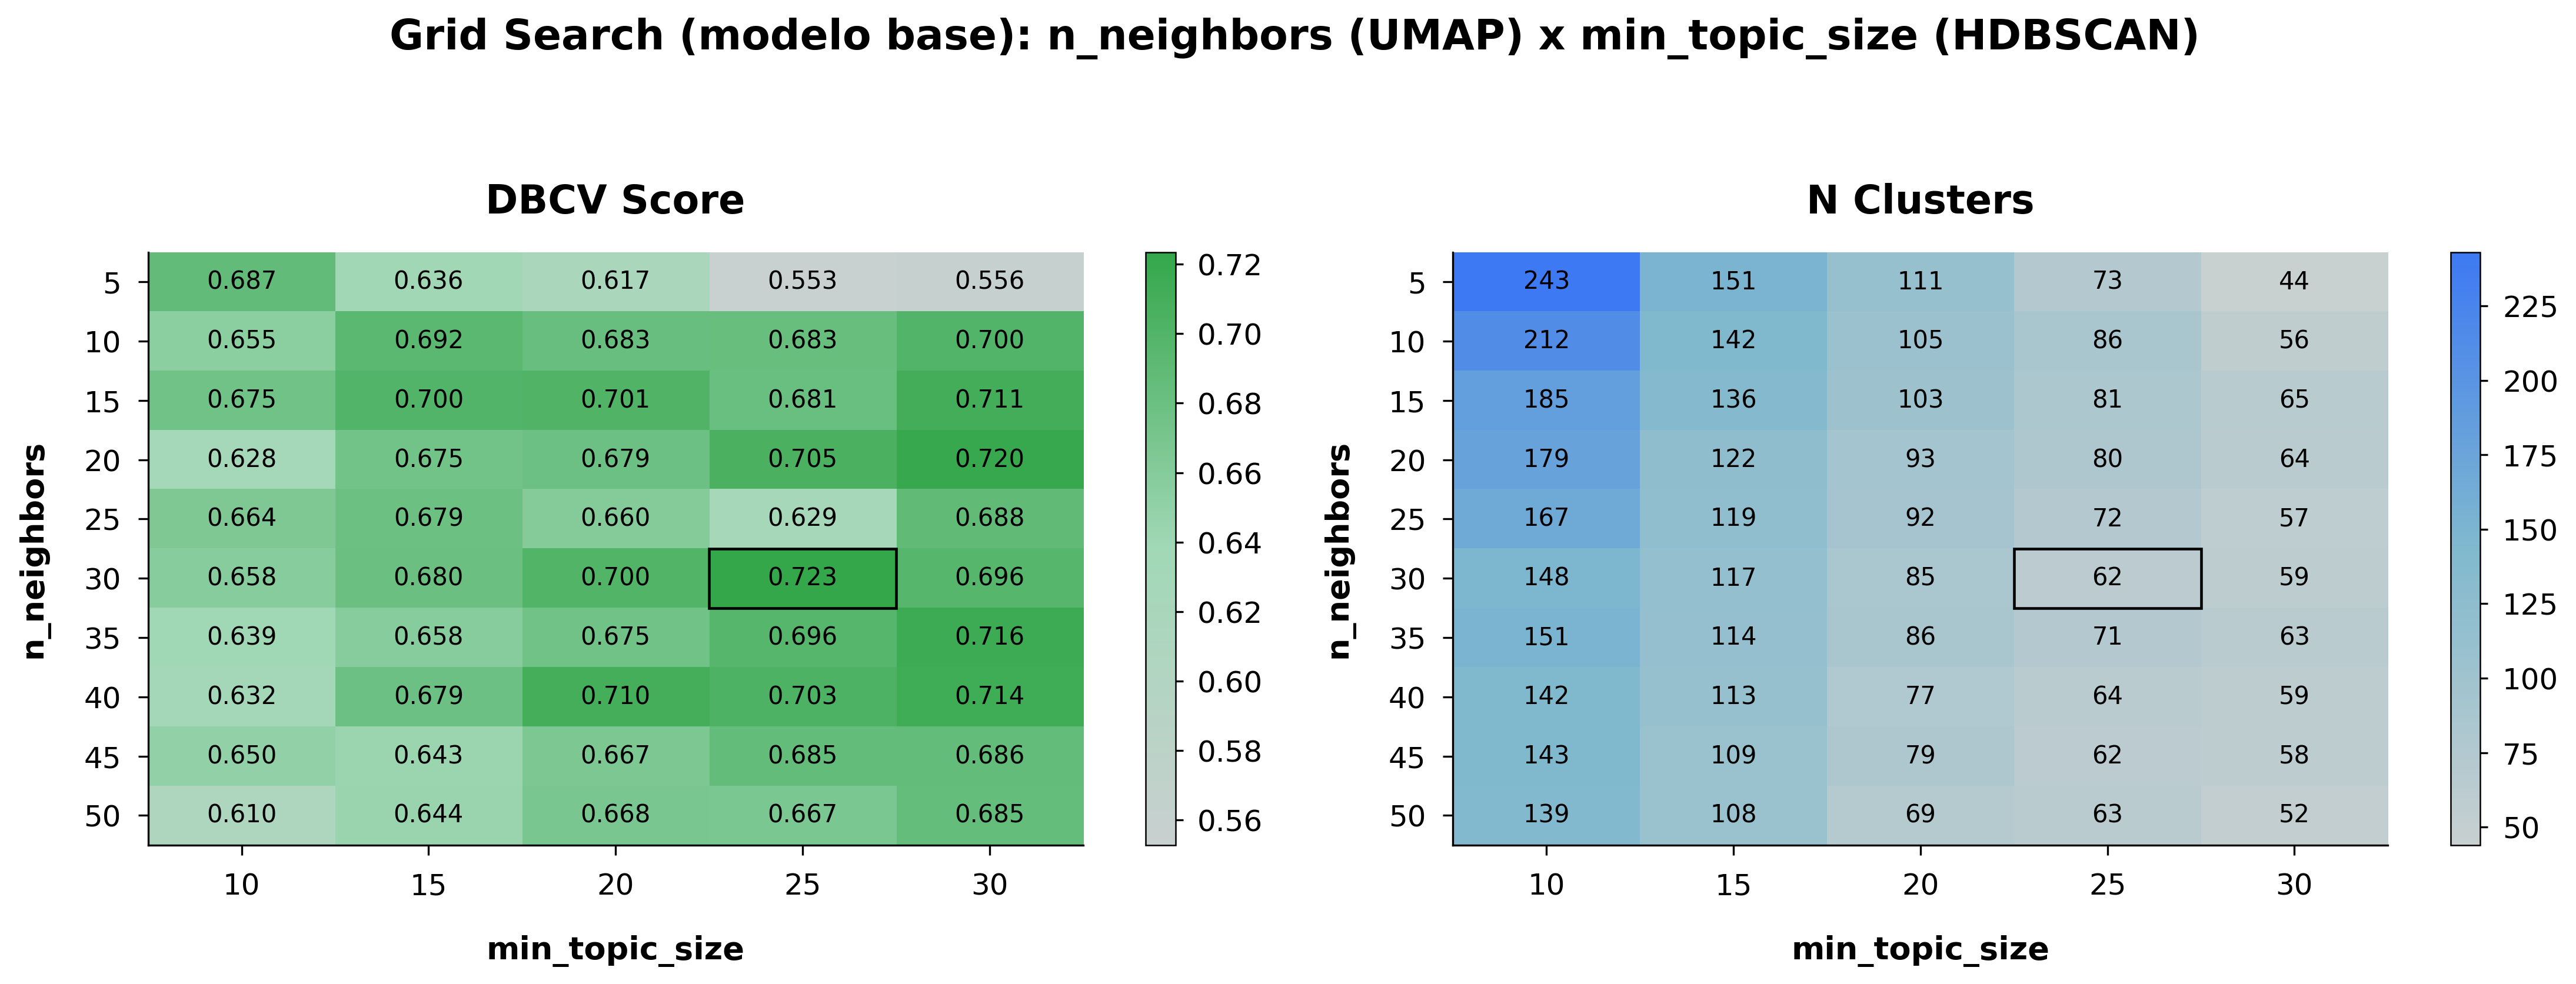
\includegraphics[width=\textwidth]{umap_param_grid_search_base.png}
  \fonte{Elaborado pelos autores.}
\end{figure}

\FloatBarrier

\subsection{BERTopic Passagem 1 e Fine-Tuning}

Com os hiperparâmetros ótimos, a primeira passagem do BERTopic produz 62 clusters. Esses clusters não são os rótulos finais, mas servem como fonte de pares positivos para o fine-tuning contrastivo do modelo de embeddings.

O fine-tuning usa \textit{MultipleNegativesRankingLoss} \cite{karpukhin2020dpr,gao2021simcse}: dois textos no mesmo cluster formam um par positivo e os demais positivos no mesmo batch atuam como negativos implícitos. O objetivo é aproximar textos semanticamente equivalentes no espaço de embeddings e afastar textos de infrações diferentes. O ajuste é feito por uma época, e o modelo resultante é salvo para reutilização.

\subsection{BERTopic Passagem 2}

Um segundo grid search é executado sobre os embeddings do modelo fine-tunado, pois a geometria do espaço muda após o ajuste. A Passagem~2 produz 79 clusters com melhor separação, confirmada pelo ganho de 21,7\% no DBCV.

\subsection{Taxonomia Manual}

O BERTopic agrupa os textos, mas a decisão semântica final é uma taxonomia manual que mapeia os 79 clusters em 18 grupos disciplinares correspondentes às Leis do Jogo da IFAB. A atribuição segue três camadas: mapeamento direto de cluster para grupo, âncoras lexicais de alta precisão que corrigem clusters mistos, e um fallback auditável para textos outliers. As âncoras cobrem termos determinísticos como ``temerária'', ``força excessiva'', ``oportunidade clara de gol'', ``simulação'' e ``mão na bola''. No total, 6.069 ajustes por âncoras foram aplicados.


\section{Critérios de Avaliação}

Os dois métodos são comparados por dois critérios complementares, aplicados independentemente a cada conjunto de rótulos.

O primeiro critério é o \textbf{score de coesão semântica}. Para cada texto, calcula-se a similaridade de cosseno entre seu embedding e o centroide ponderado do grupo ao qual foi atribuído. O score médio por grupo indica o quão compactos e internamente coesos são os textos reunidos sob aquela categoria. Valores altos significam que o modelo de embeddings percebe os textos do grupo como semanticamente próximos, enquanto valores baixos indicam grupos com vocabulário mais heterogêneo.

O segundo critério é a \textbf{recuperabilidade}, avaliada no Notebook~4. Os rótulos atribuídos por cada método são tratados como verdade e utilizados para treinar classificadores em validação cruzada com 5 folds estratificados, usando os embeddings fine-tunados como único atributo. Três classificadores são avaliados: KNN, Regressão Logística e SVM Linear \cite{cortes1995svm,pedregosa2011sklearn}. A ideia é que rótulos semanticamente coerentes no espaço de embeddings devem ser recuperáveis por um classificador simples com alta precisão. As métricas reportadas são F1 Macro e Accuracy.

Juntos, os dois critérios cobrem perspectivas distintas: o score de coesão mede a compactidade interna de cada grupo individualmente, enquanto a recuperabilidade avalia se os grupos são separáveis entre si no espaço de embeddings.

% =============================================================================
\chapter{Resultados}
% =============================================================================

\section{Análise Exploratória dos Cartões}

A base modelada contém 25.834 cartões: 24.897 amarelos (96,4\%) e 937 vermelhos (3,6\%), distribuídos em 248 times e com 173 árbitros distintos. A Figura~\ref{fig-cards-year} mostra a distribuição anual por tipo de cartão.

\begin{figure}[!htp]
  \centering
  \caption{Volume de cartões por ano e tipo.}
  \label{fig-cards-year}
  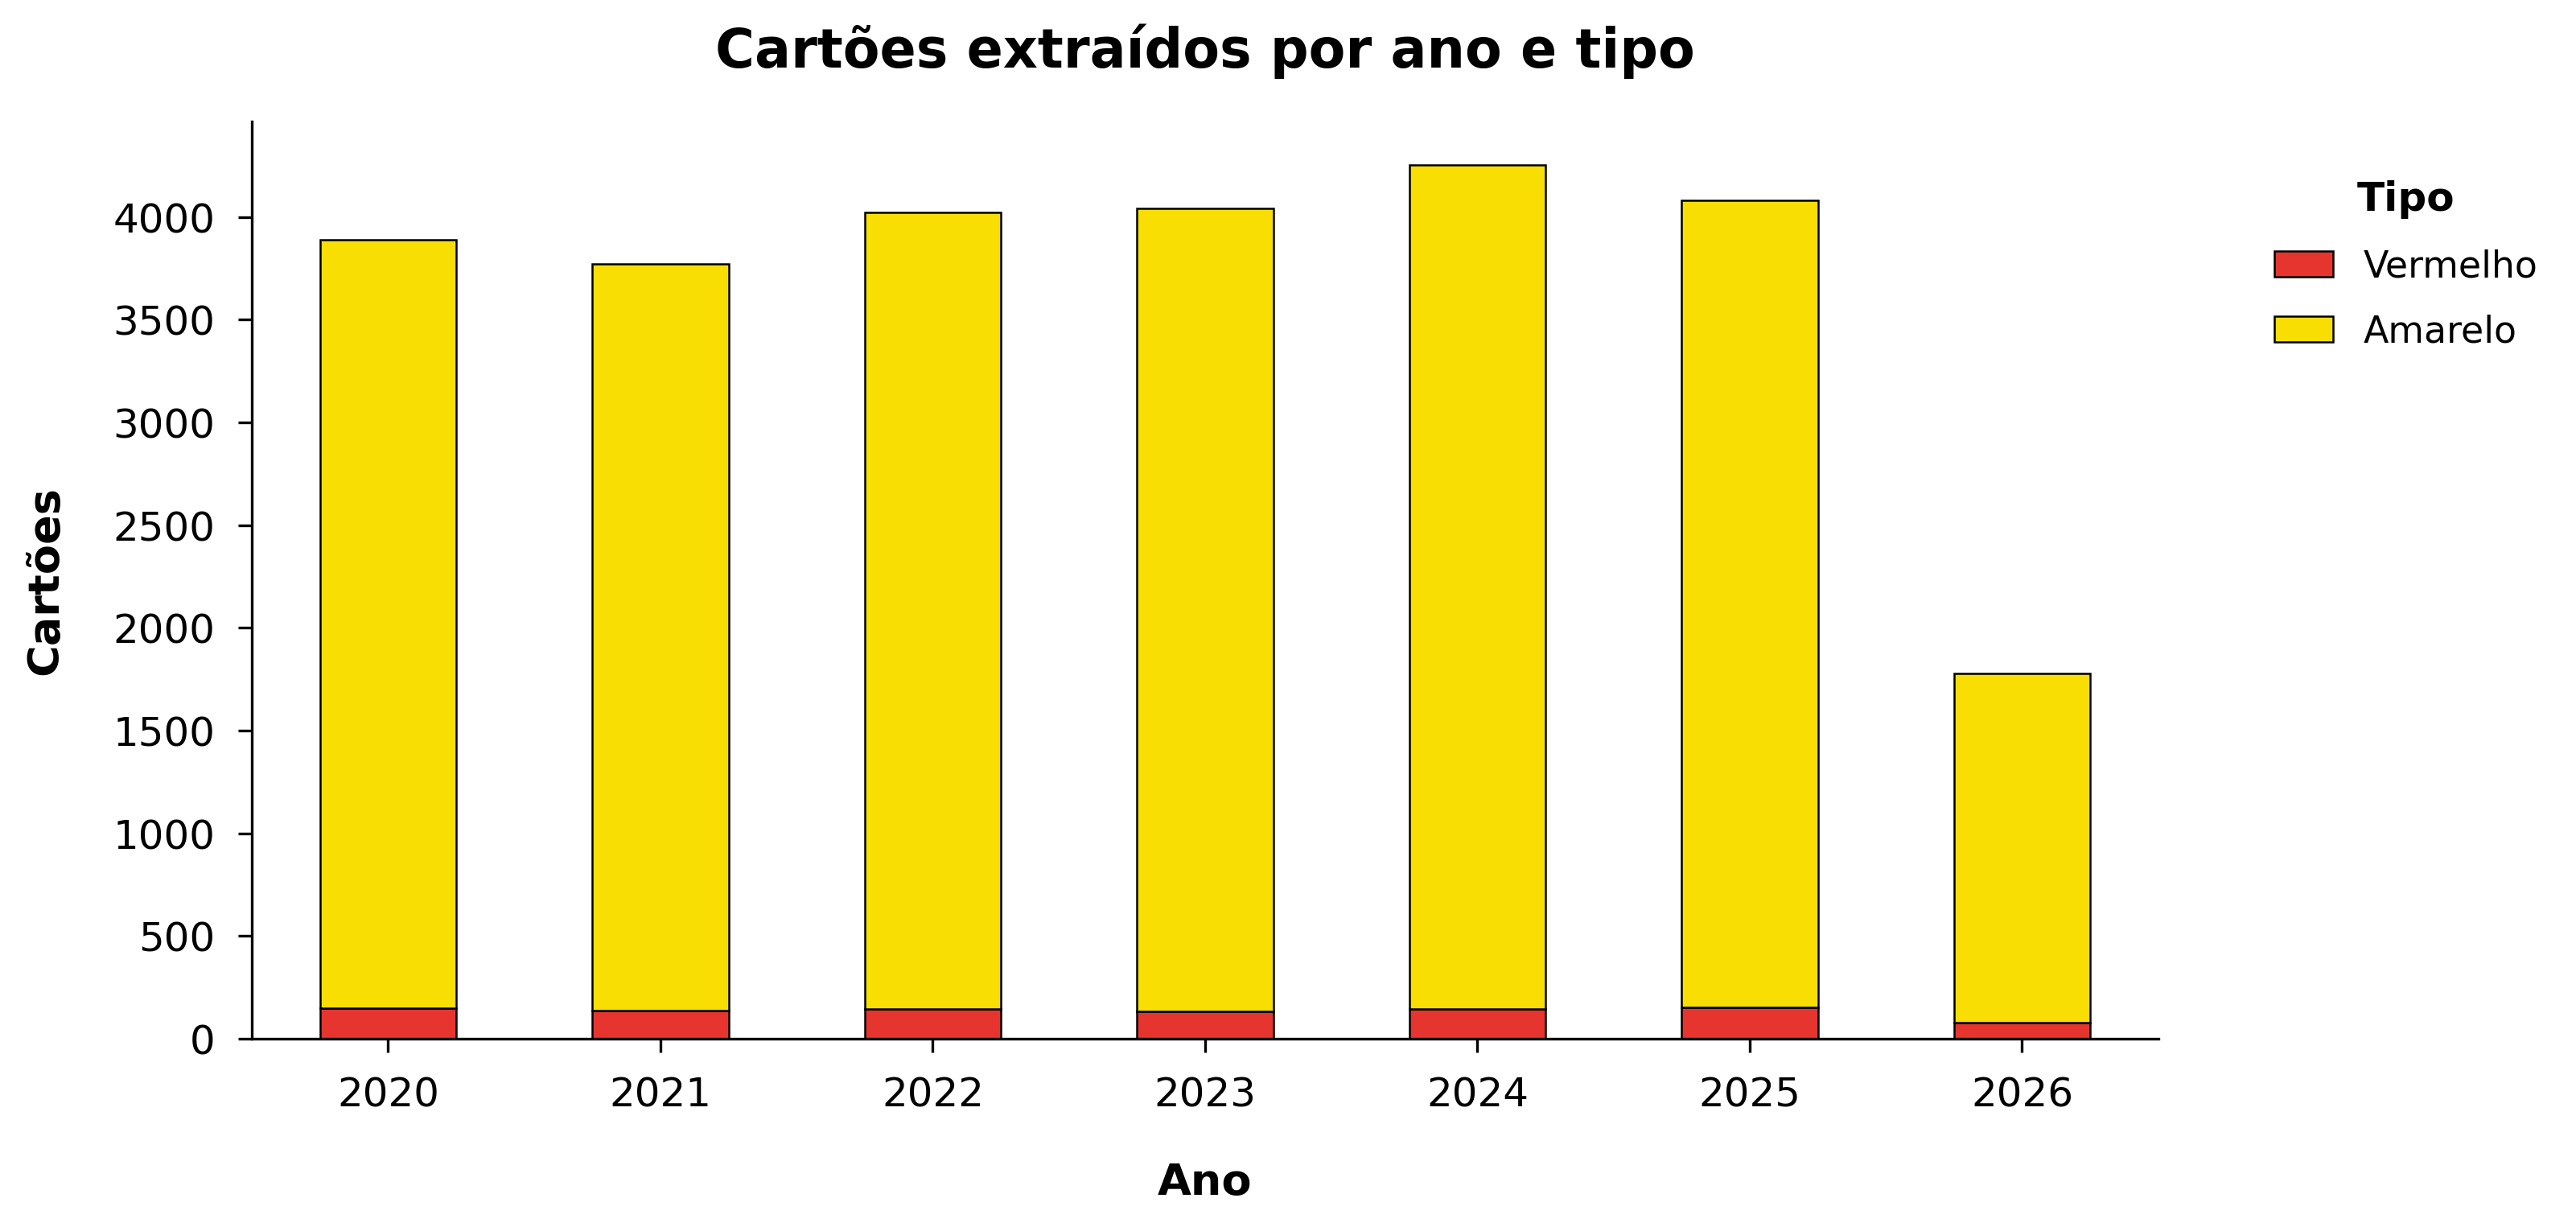
\includegraphics[width=0.90\textwidth]{cards_by_year_type.png}
  \fonte{Elaborado pelos autores.}
\end{figure}

\FloatBarrier

O volume é estável entre 2020 e 2025, com cerca de 3.880 amarelos por ano. O ano de 2026 é parcial. A Figura~\ref{fig-top-texts} mostra os textos de justificativa mais frequentes, revelando que variações de ``calçar o adversário de maneira temerária'' e ``falta tática impedindo ataque promissor'' dominam o corpus. Essa concentração em poucos padrões coexiste com alta diversidade lexical nos 6.945 textos únicos, o que justifica o uso de embeddings densos em vez de correspondência lexical direta.

\begin{figure}[!htp]
  \centering
  \caption{Textos de justificativa de cartão mais frequentes.}
  \label{fig-top-texts}
  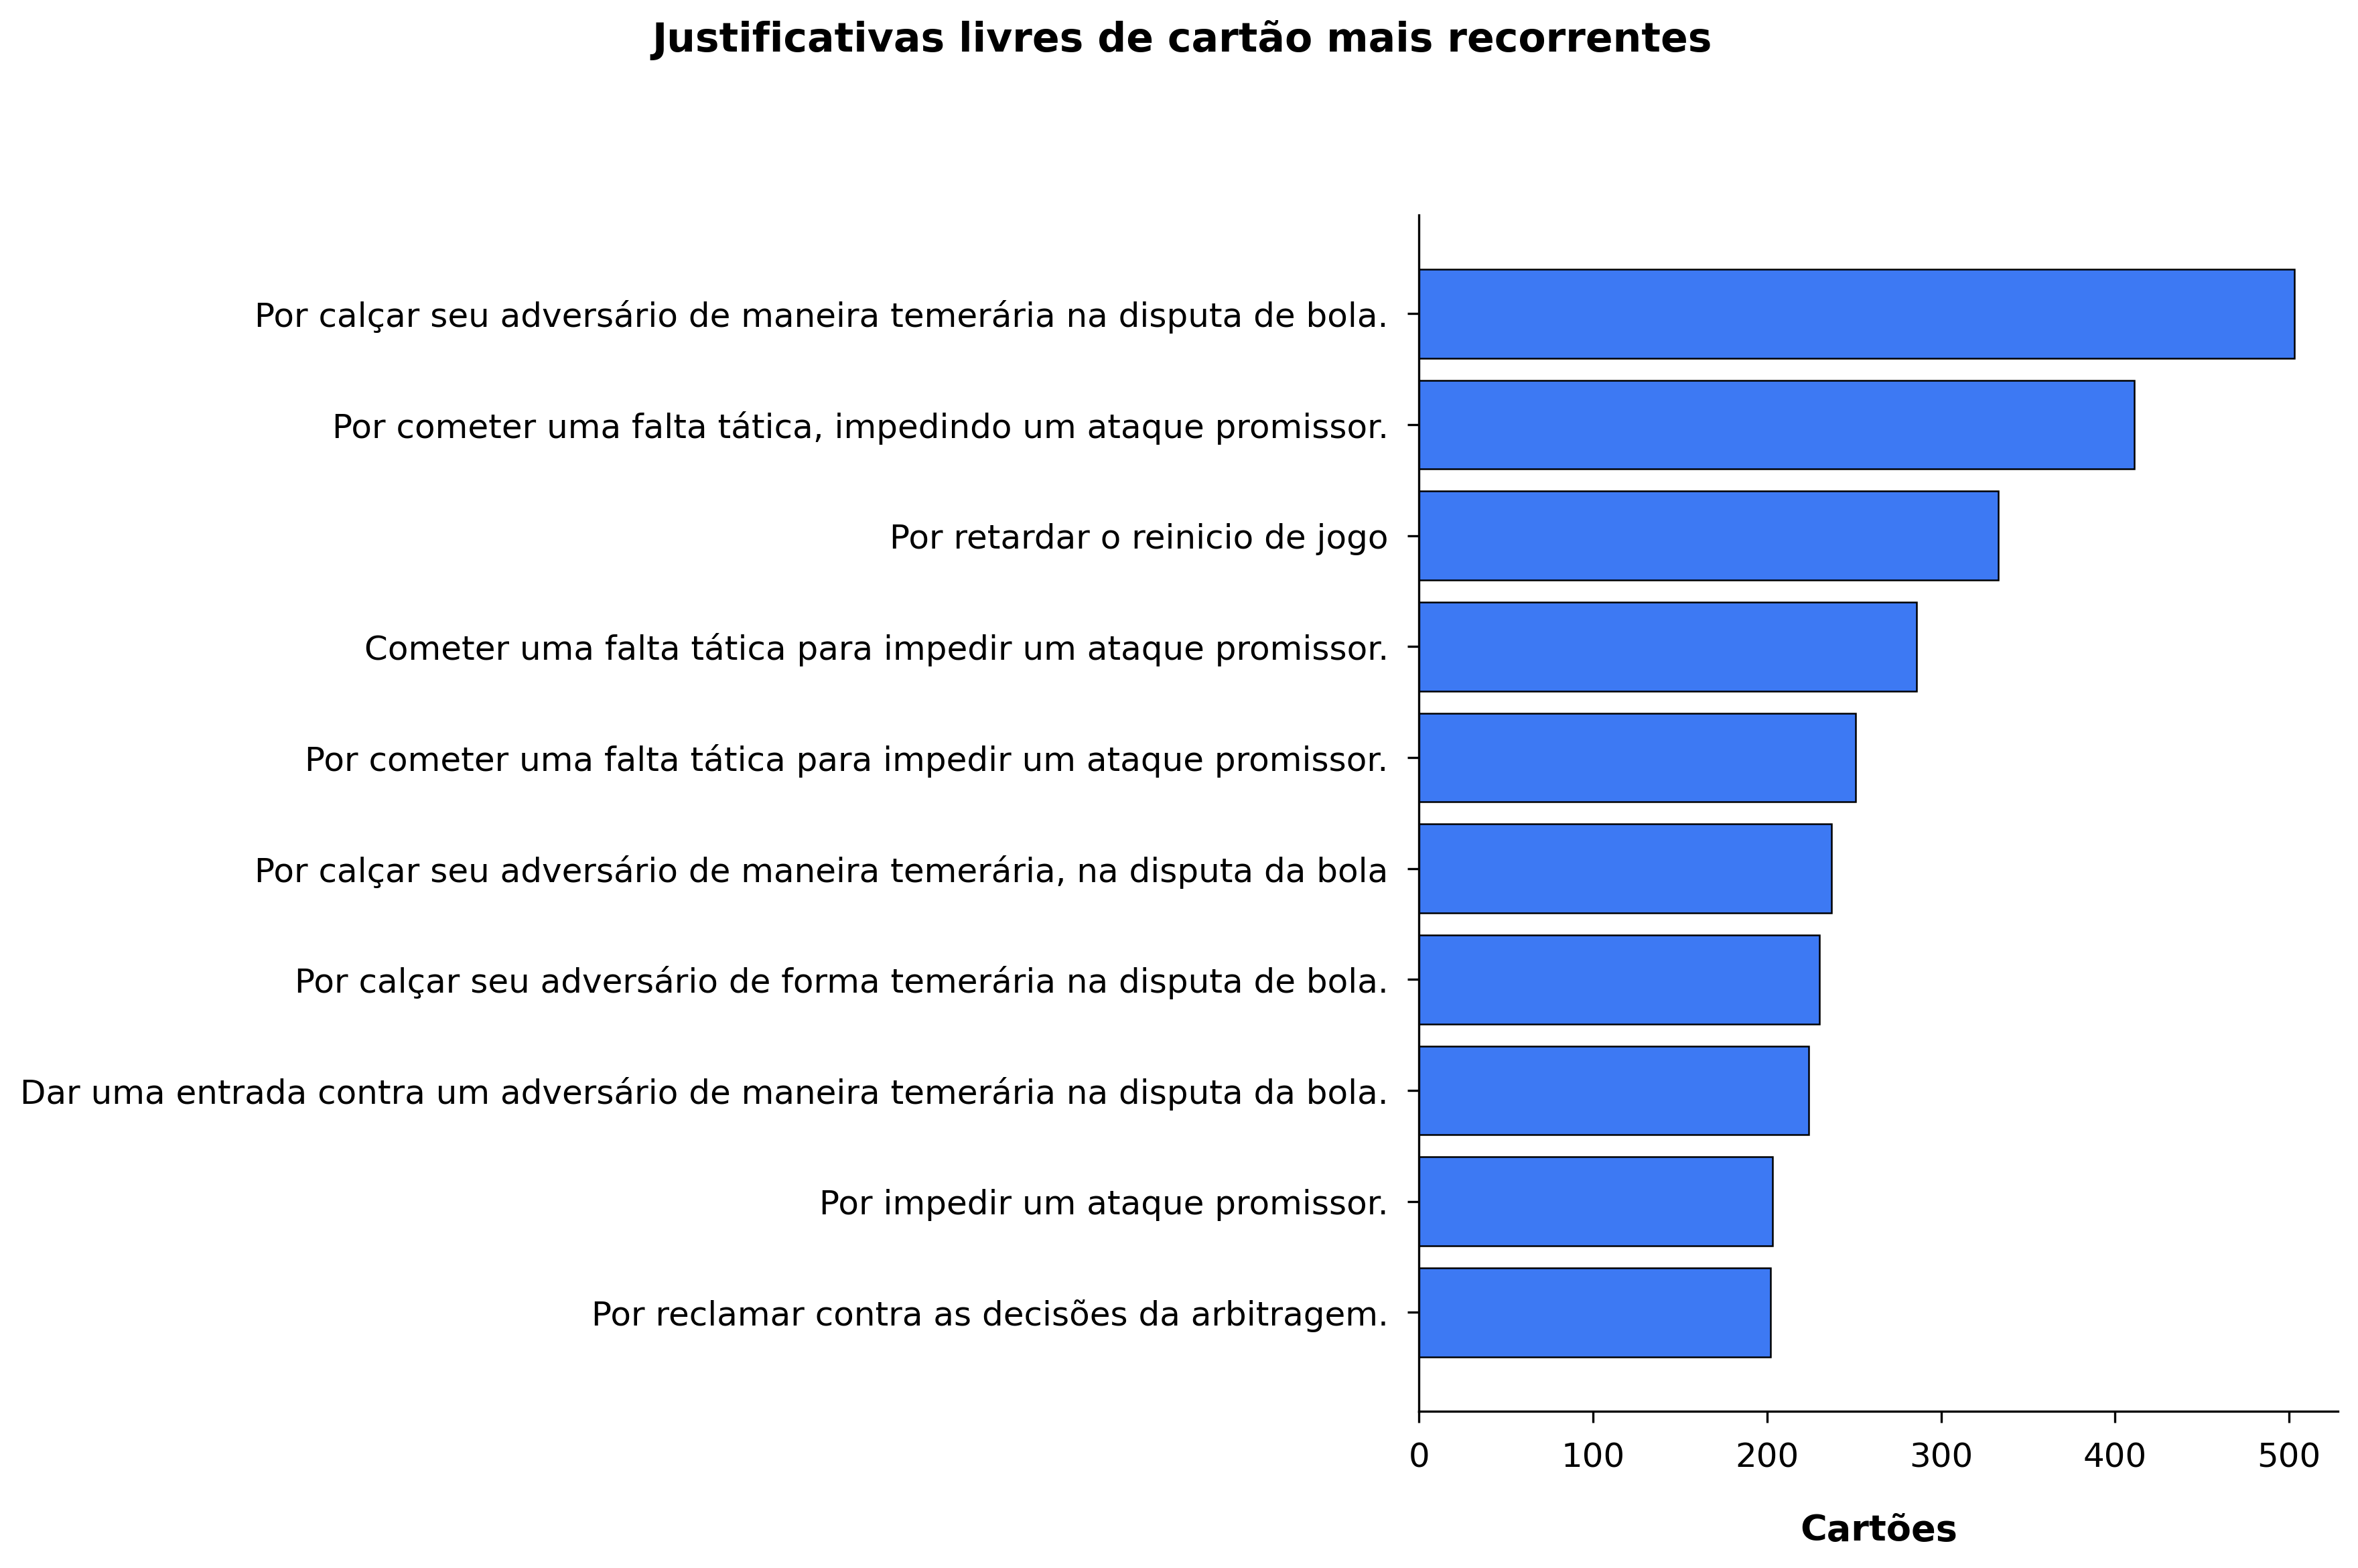
\includegraphics[width=0.90\textwidth]{top_card_reason_texts.png}
  \fonte{Elaborado pelos autores.}
\end{figure}

\FloatBarrier

\section{Efeito do Fine-Tuning}

A Tabela~\ref{tab-ablation} resume os indicadores das duas passagens. A Figura~\ref{fig-ablation} ilustra a comparação.

\begin{table}[!htp]
  \centering
  \caption{Ablação: modelo base versus modelo fine-tunado.}
  \label{tab-ablation}
  \begin{tabular}{lrrrr}
    \toprule
    Passagem & Clusters & Outliers & Outliers (\%) & DBCV \\
    \midrule
    Passagem 1 (base) & 62 & 938 & 13,5 & 0,7235 \\
    Passagem 2 (fine-tunado) & 79 & 504 & 7,3 & 0,8806 \\
    \bottomrule
  \end{tabular}
  \fonte{Elaborado pelos autores.}
  \nota{Ganho em DBCV: $+$21,7\%. Redução de outliers: $-$6,2 pontos percentuais.}
\end{table}

\begin{figure}[!htp]
  \centering
  \caption{Ablação: desempenho de clustering por passagem do pipeline.}
  \label{fig-ablation}
  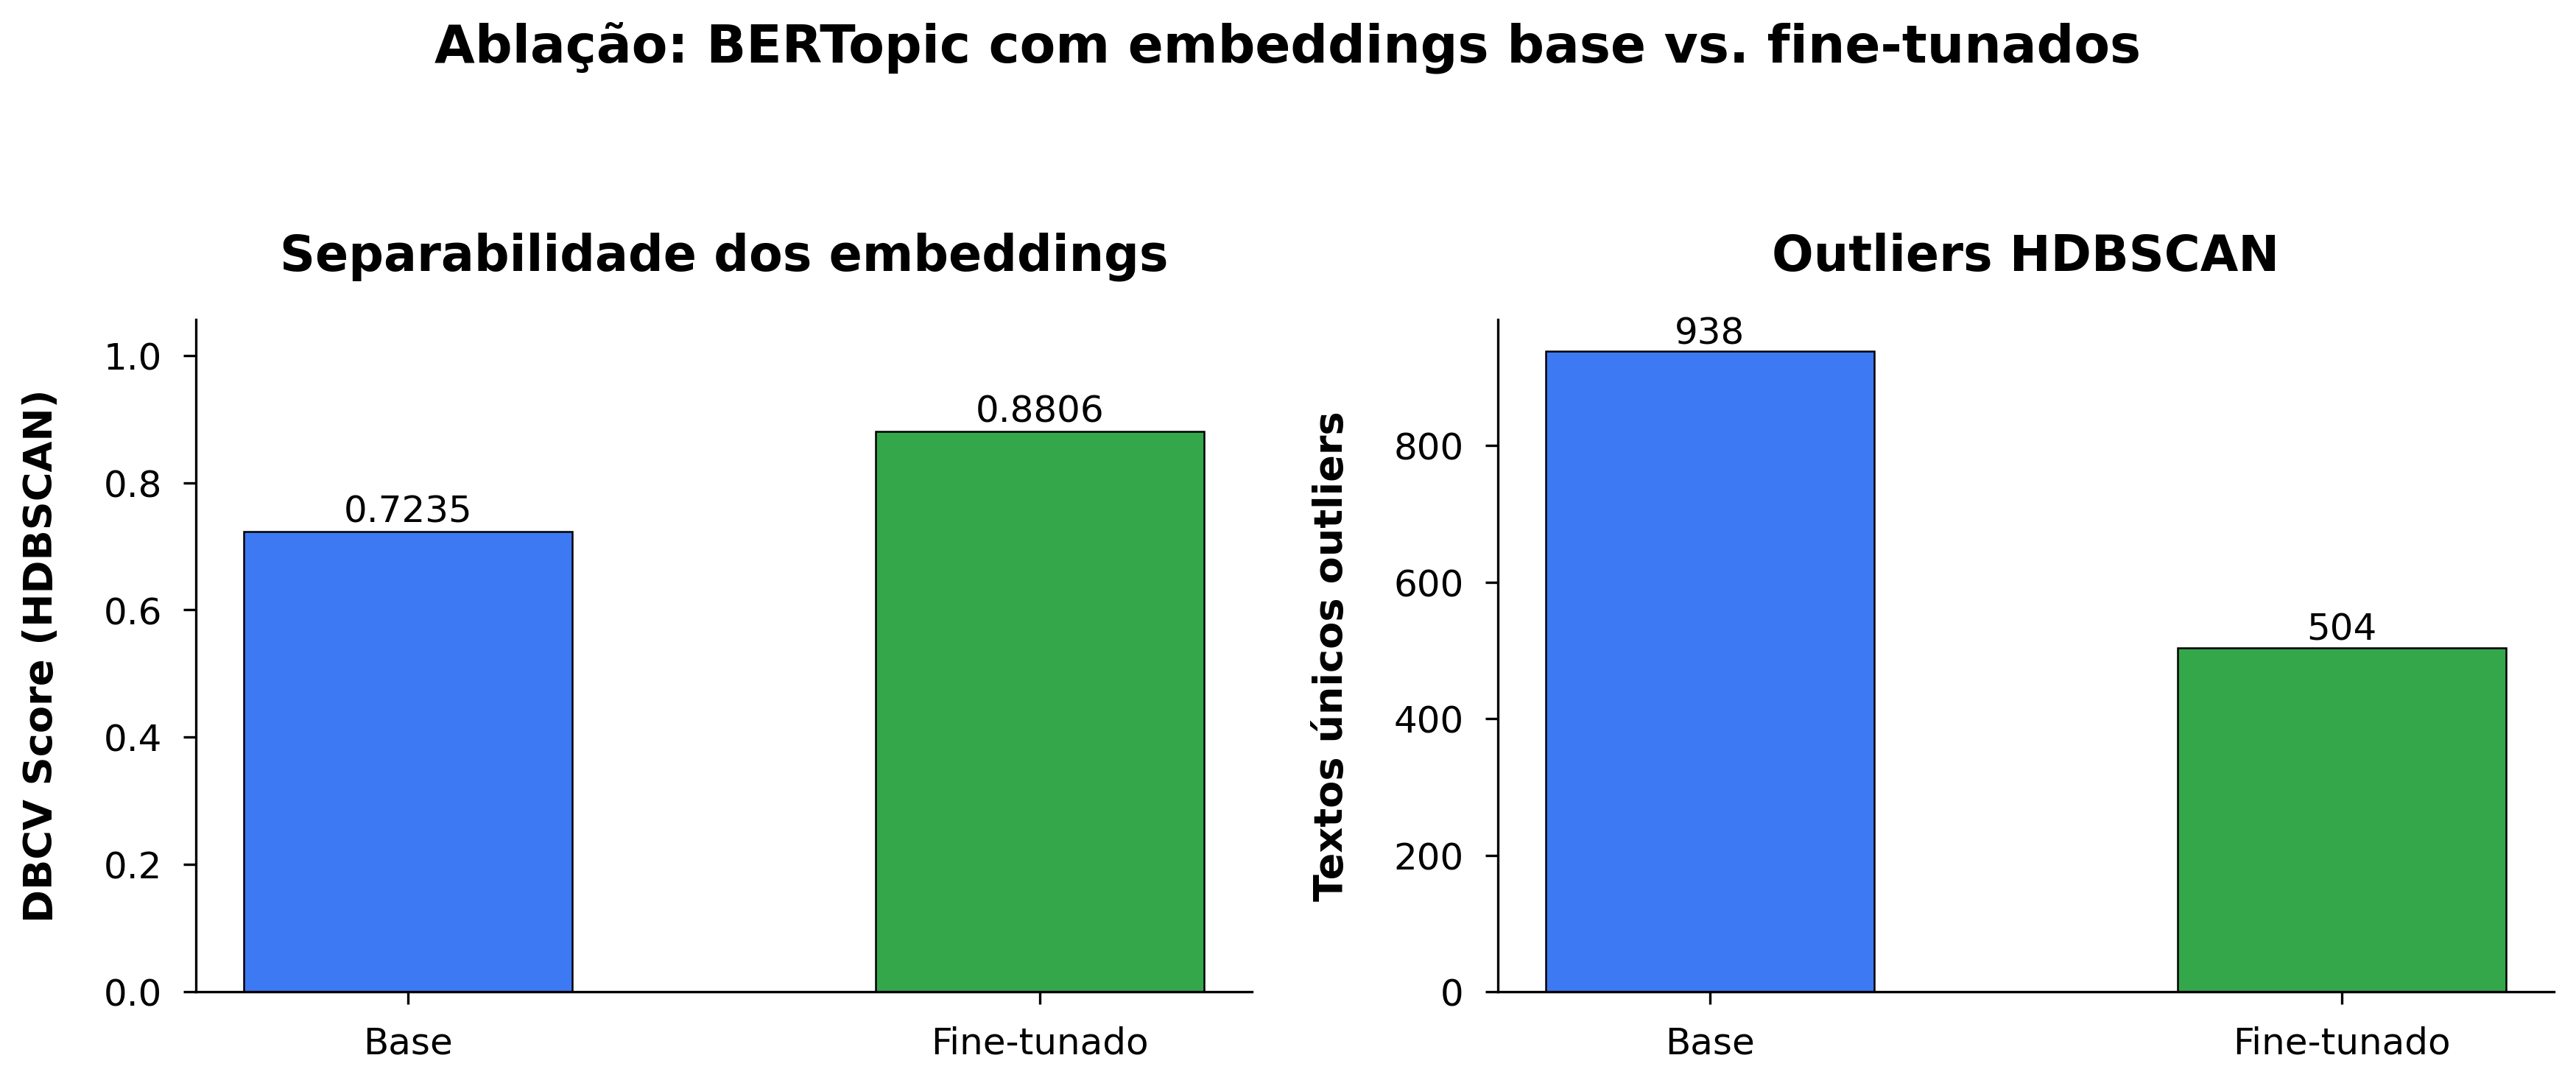
\includegraphics[width=0.82\textwidth]{ablation_dbcv.png}
  \fonte{Elaborado pelos autores.}
\end{figure}

\FloatBarrier

O fine-tuning reduz a taxa de outliers em 6,2 pontos percentuais e aumenta o DBCV em 21,7\%. O maior número de clusters na Passagem~2 reflete a maior resolução do espaço após o ajuste, com subgrupos antes misturados sendo separados em regiões densas distintas.

\section{Taxonomia Final: 18 Grupos Disciplinares}

A Figura~\ref{fig-counts} mostra a distribuição de cartões por grupo e a Tabela~\ref{tab-grupos} detalha os 18 grupos.

\begin{figure}[!htp]
  \centering
  \caption{Distribuição de cartões por grupo disciplinar.}
  \label{fig-counts}
  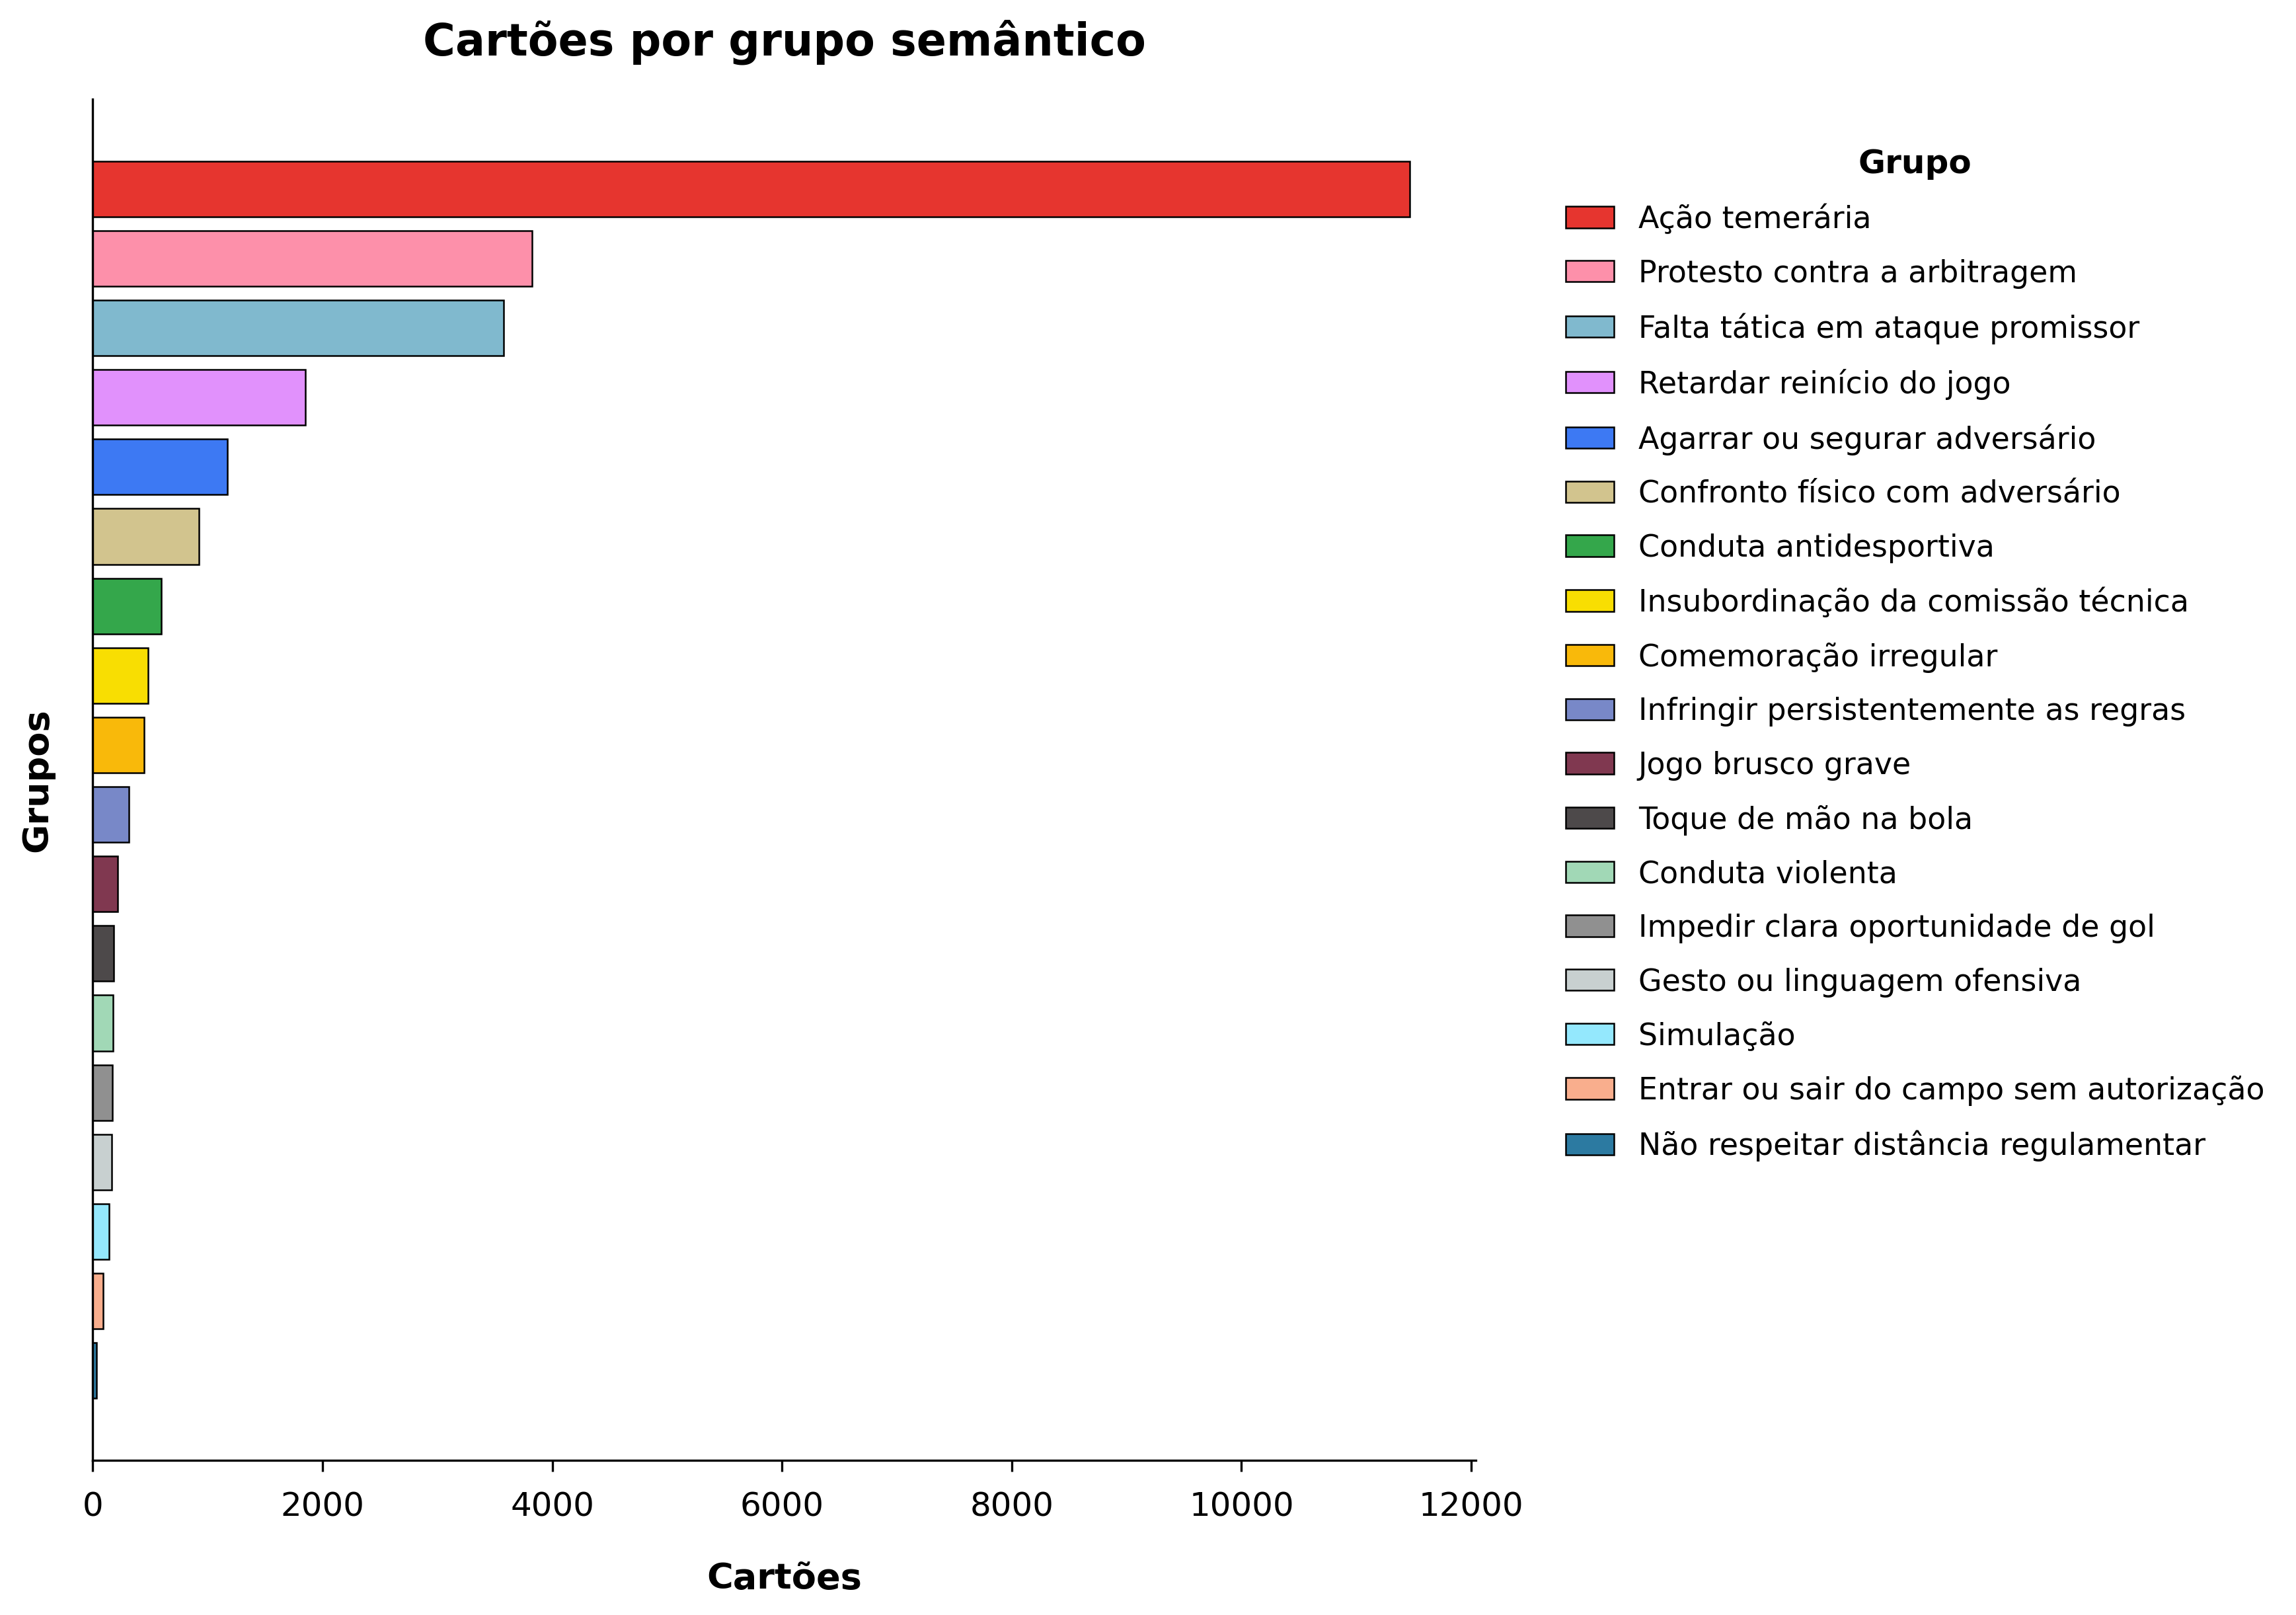
\includegraphics[width=0.75\textwidth]{card_reason_groups_counts.png}
  \fonte{Elaborado pelos autores.}
\end{figure}

\FloatBarrier

\begin{table}[!htp]
  \centering
  \caption{Distribuição dos 18 grupos disciplinares.}
  \label{tab-grupos}
  \small
  \begin{tabular}{lrr}
    \toprule
    Grupo & Cartões & \% \\
    \midrule
    Ação temerária & 11.465 & 44,4 \\
    Protesto contra a arbitragem & 3.825 & 14,8 \\
    Falta tática em ataque promissor & 3.575 & 13,8 \\
    Retardar reinício do jogo & 1.852 & 7,2 \\
    Agarrar ou segurar adversário & 1.174 & 4,5 \\
    Confronto físico com adversário & 927 & 3,6 \\
    Conduta antidesportiva & 595 & 2,3 \\
    Insubordinação da comissão técnica & 483 & 1,9 \\
    Comemoração irregular & 447 & 1,7 \\
    Infringir persistentemente as regras & 314 & 1,2 \\
    Jogo brusco grave & 218 & 0,8 \\
    Toque de mão na bola & 184 & 0,7 \\
    Conduta violenta & 176 & 0,7 \\
    Gesto ou linguagem ofensiva & 165 & 0,6 \\
    Impedir clara oportunidade de gol & 171 & 0,7 \\
    Simulação & 140 & 0,5 \\
    Entrar ou sair do campo sem autorização & 91 & 0,4 \\
    Não respeitar distância regulamentar & 32 & 0,1 \\
    \midrule
    Total & 25.834 & 100,0 \\
    \bottomrule
  \end{tabular}
  \fonte{Elaborado pelos autores.}
\end{table}

\FloatBarrier

Ação temerária concentra 44,4\% dos cartões, refletindo a predominância de faltas de disputa de bola. Os três grupos mais frequentes somam 72,9\% dos eventos. Grupos de menor frequência, como Não respeitar distância regulamentar e Entrar ou sair do campo sem autorização, possuem vocabulário mais específico e consequentemente maior coesão semântica.

A Figura~\ref{fig-representativeness} apresenta o score médio de coesão por grupo, medido como a similaridade de cosseno média de cada texto ao centroide ponderado do grupo no espaço de embeddings fine-tunados.

\begin{figure}[!htp]
  \centering
  \caption{Score médio de coesão semântica por grupo disciplinar.}
  \label{fig-representativeness}
  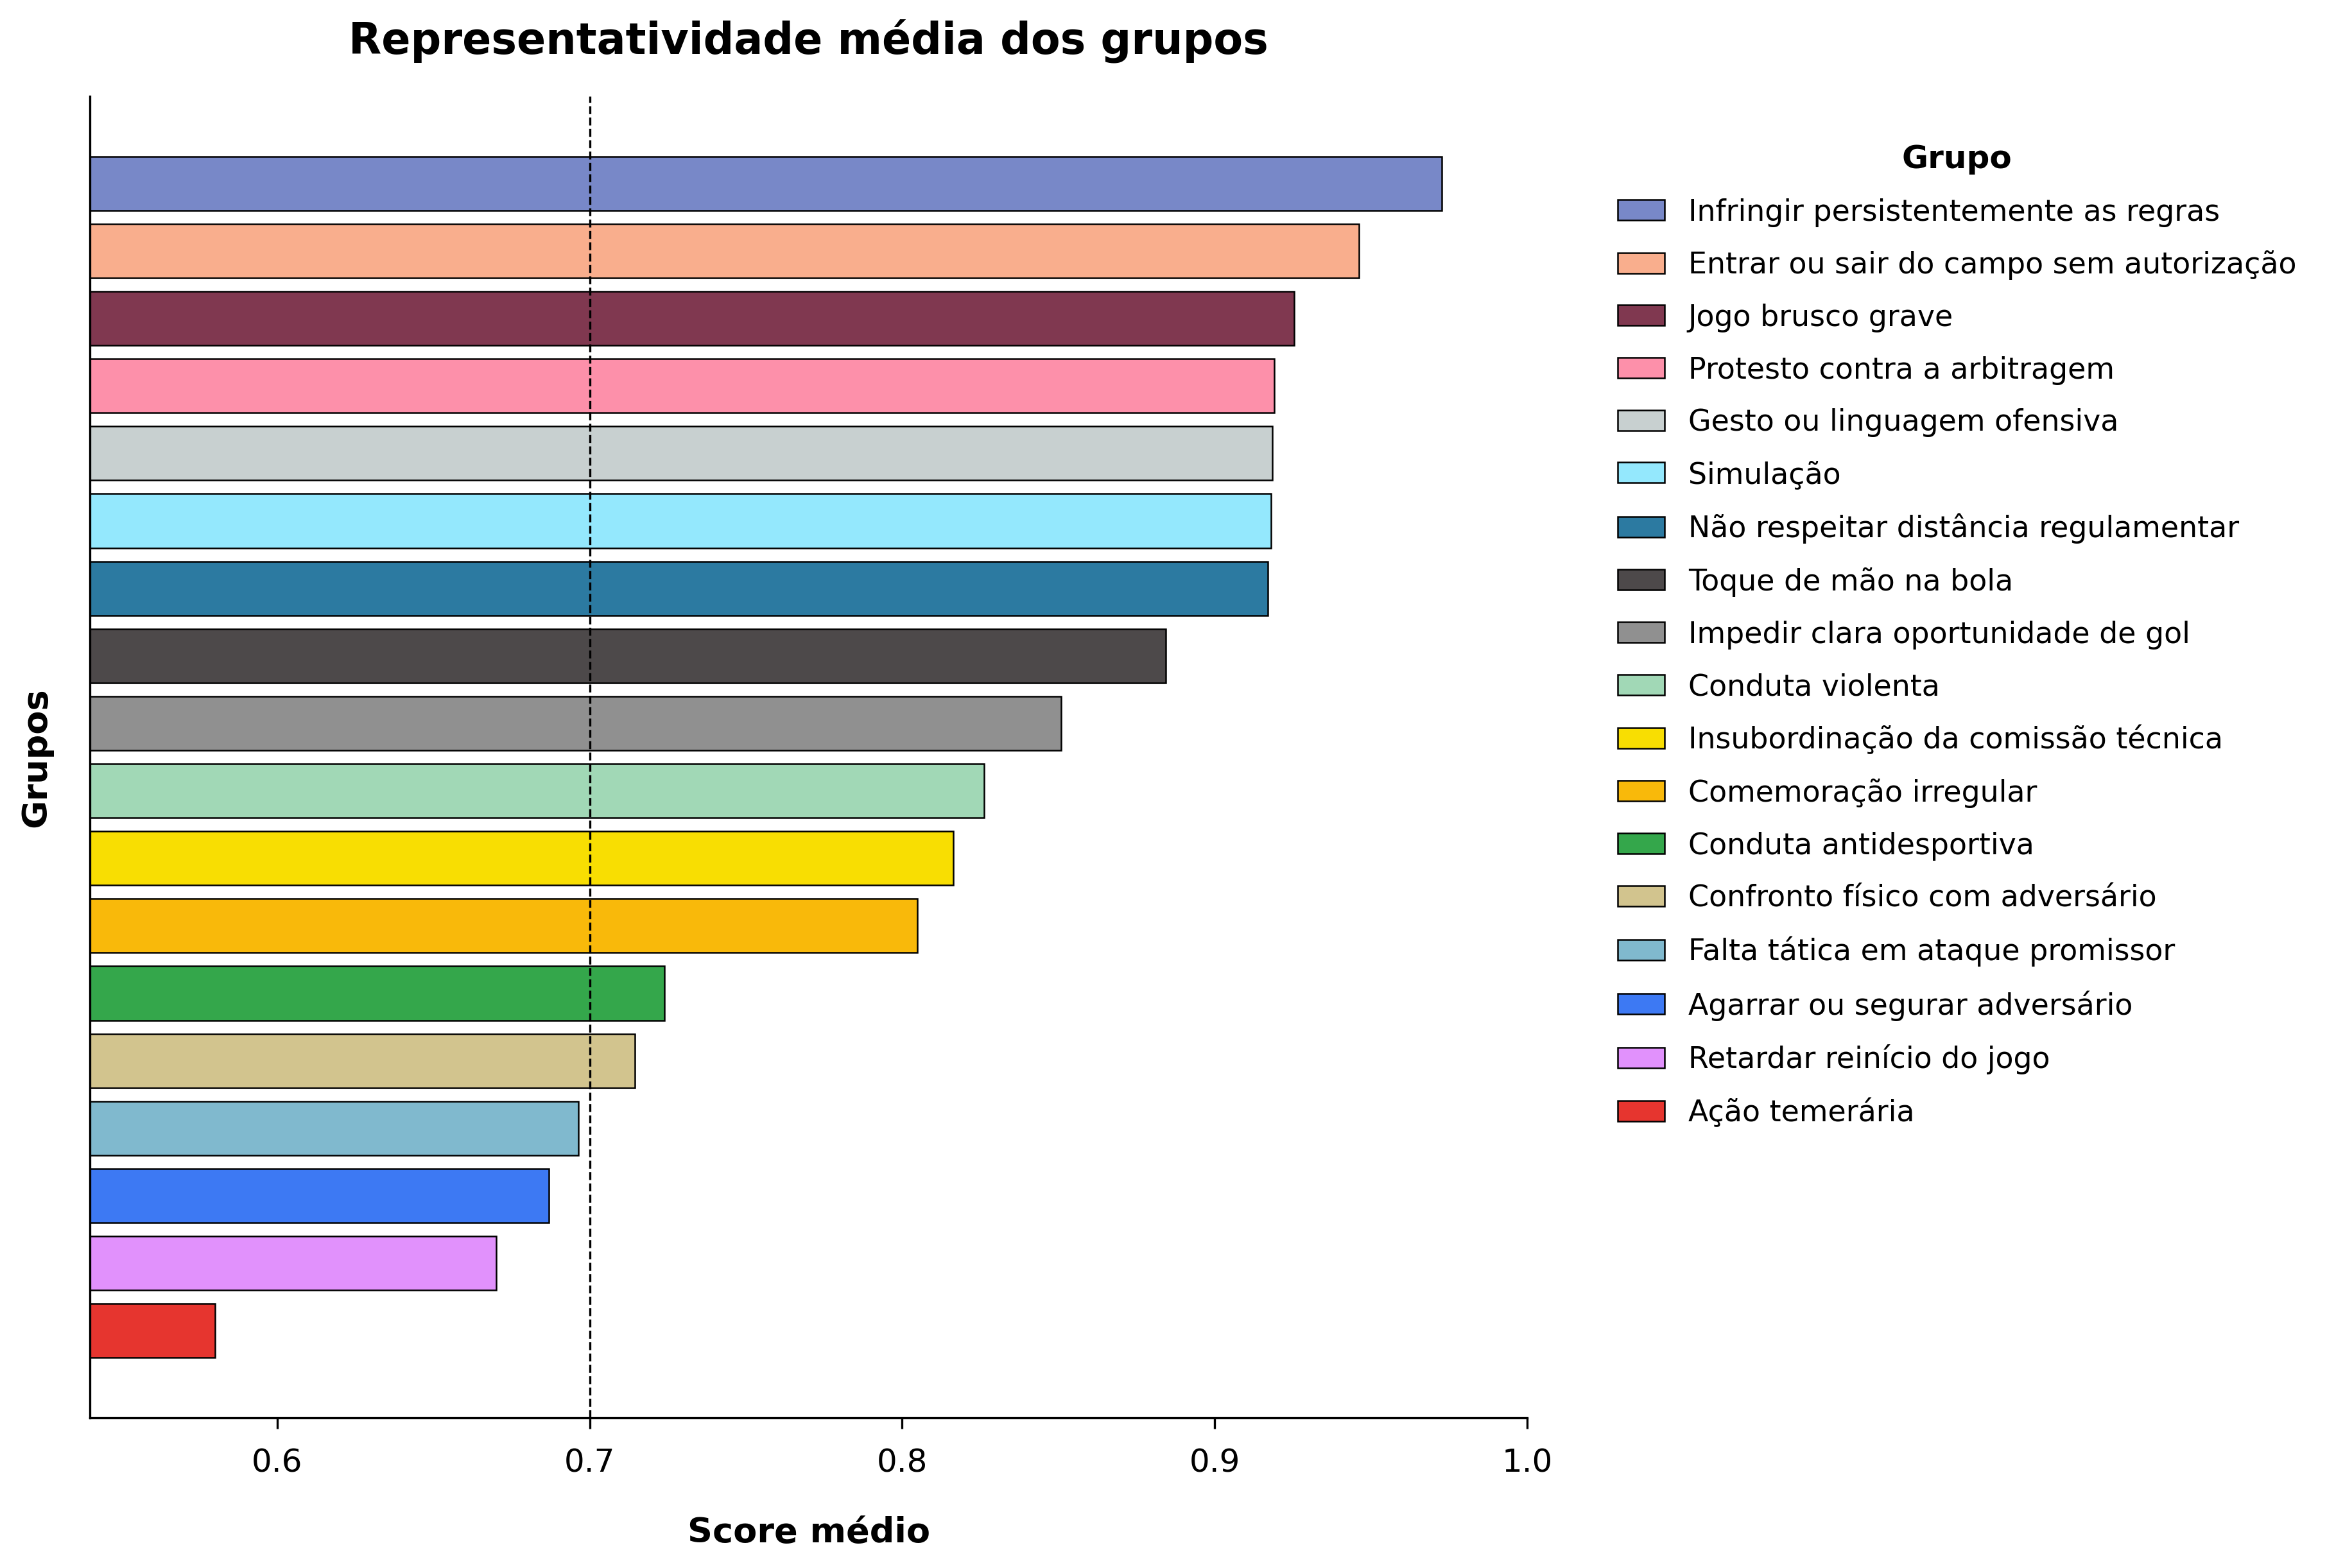
\includegraphics[width=\textwidth]{card_reason_representativeness.png}
  \fonte{Elaborado pelos autores.}
\end{figure}

\FloatBarrier

Os grupos com maior coesão são Infringir persistentemente as regras (0,973), Entrar ou sair do campo sem autorização (0,946) e Jogo brusco grave (0,925). Ação temerária, o mais frequente, tem o menor score (0,580), refletindo a alta variação lexical com que árbitros descrevem esse tipo de falta.

\section{Análise Temporal e por Perfil}

A Figura~\ref{fig-proporcoes} mostra a evolução das proporções por ano. A distribuição é relativamente estável entre 2020 e 2025. A parcela de Ação temerária apresenta leve tendência de queda, de 49,4\% em 2020 para 39,8\% em 2026, enquanto grupos como Agarrar ou segurar adversário crescem moderadamente.

\begin{figure}[!htp]
  \centering
  \caption{Proporção de cartões por grupo ao longo dos anos.}
  \label{fig-proporcoes}
  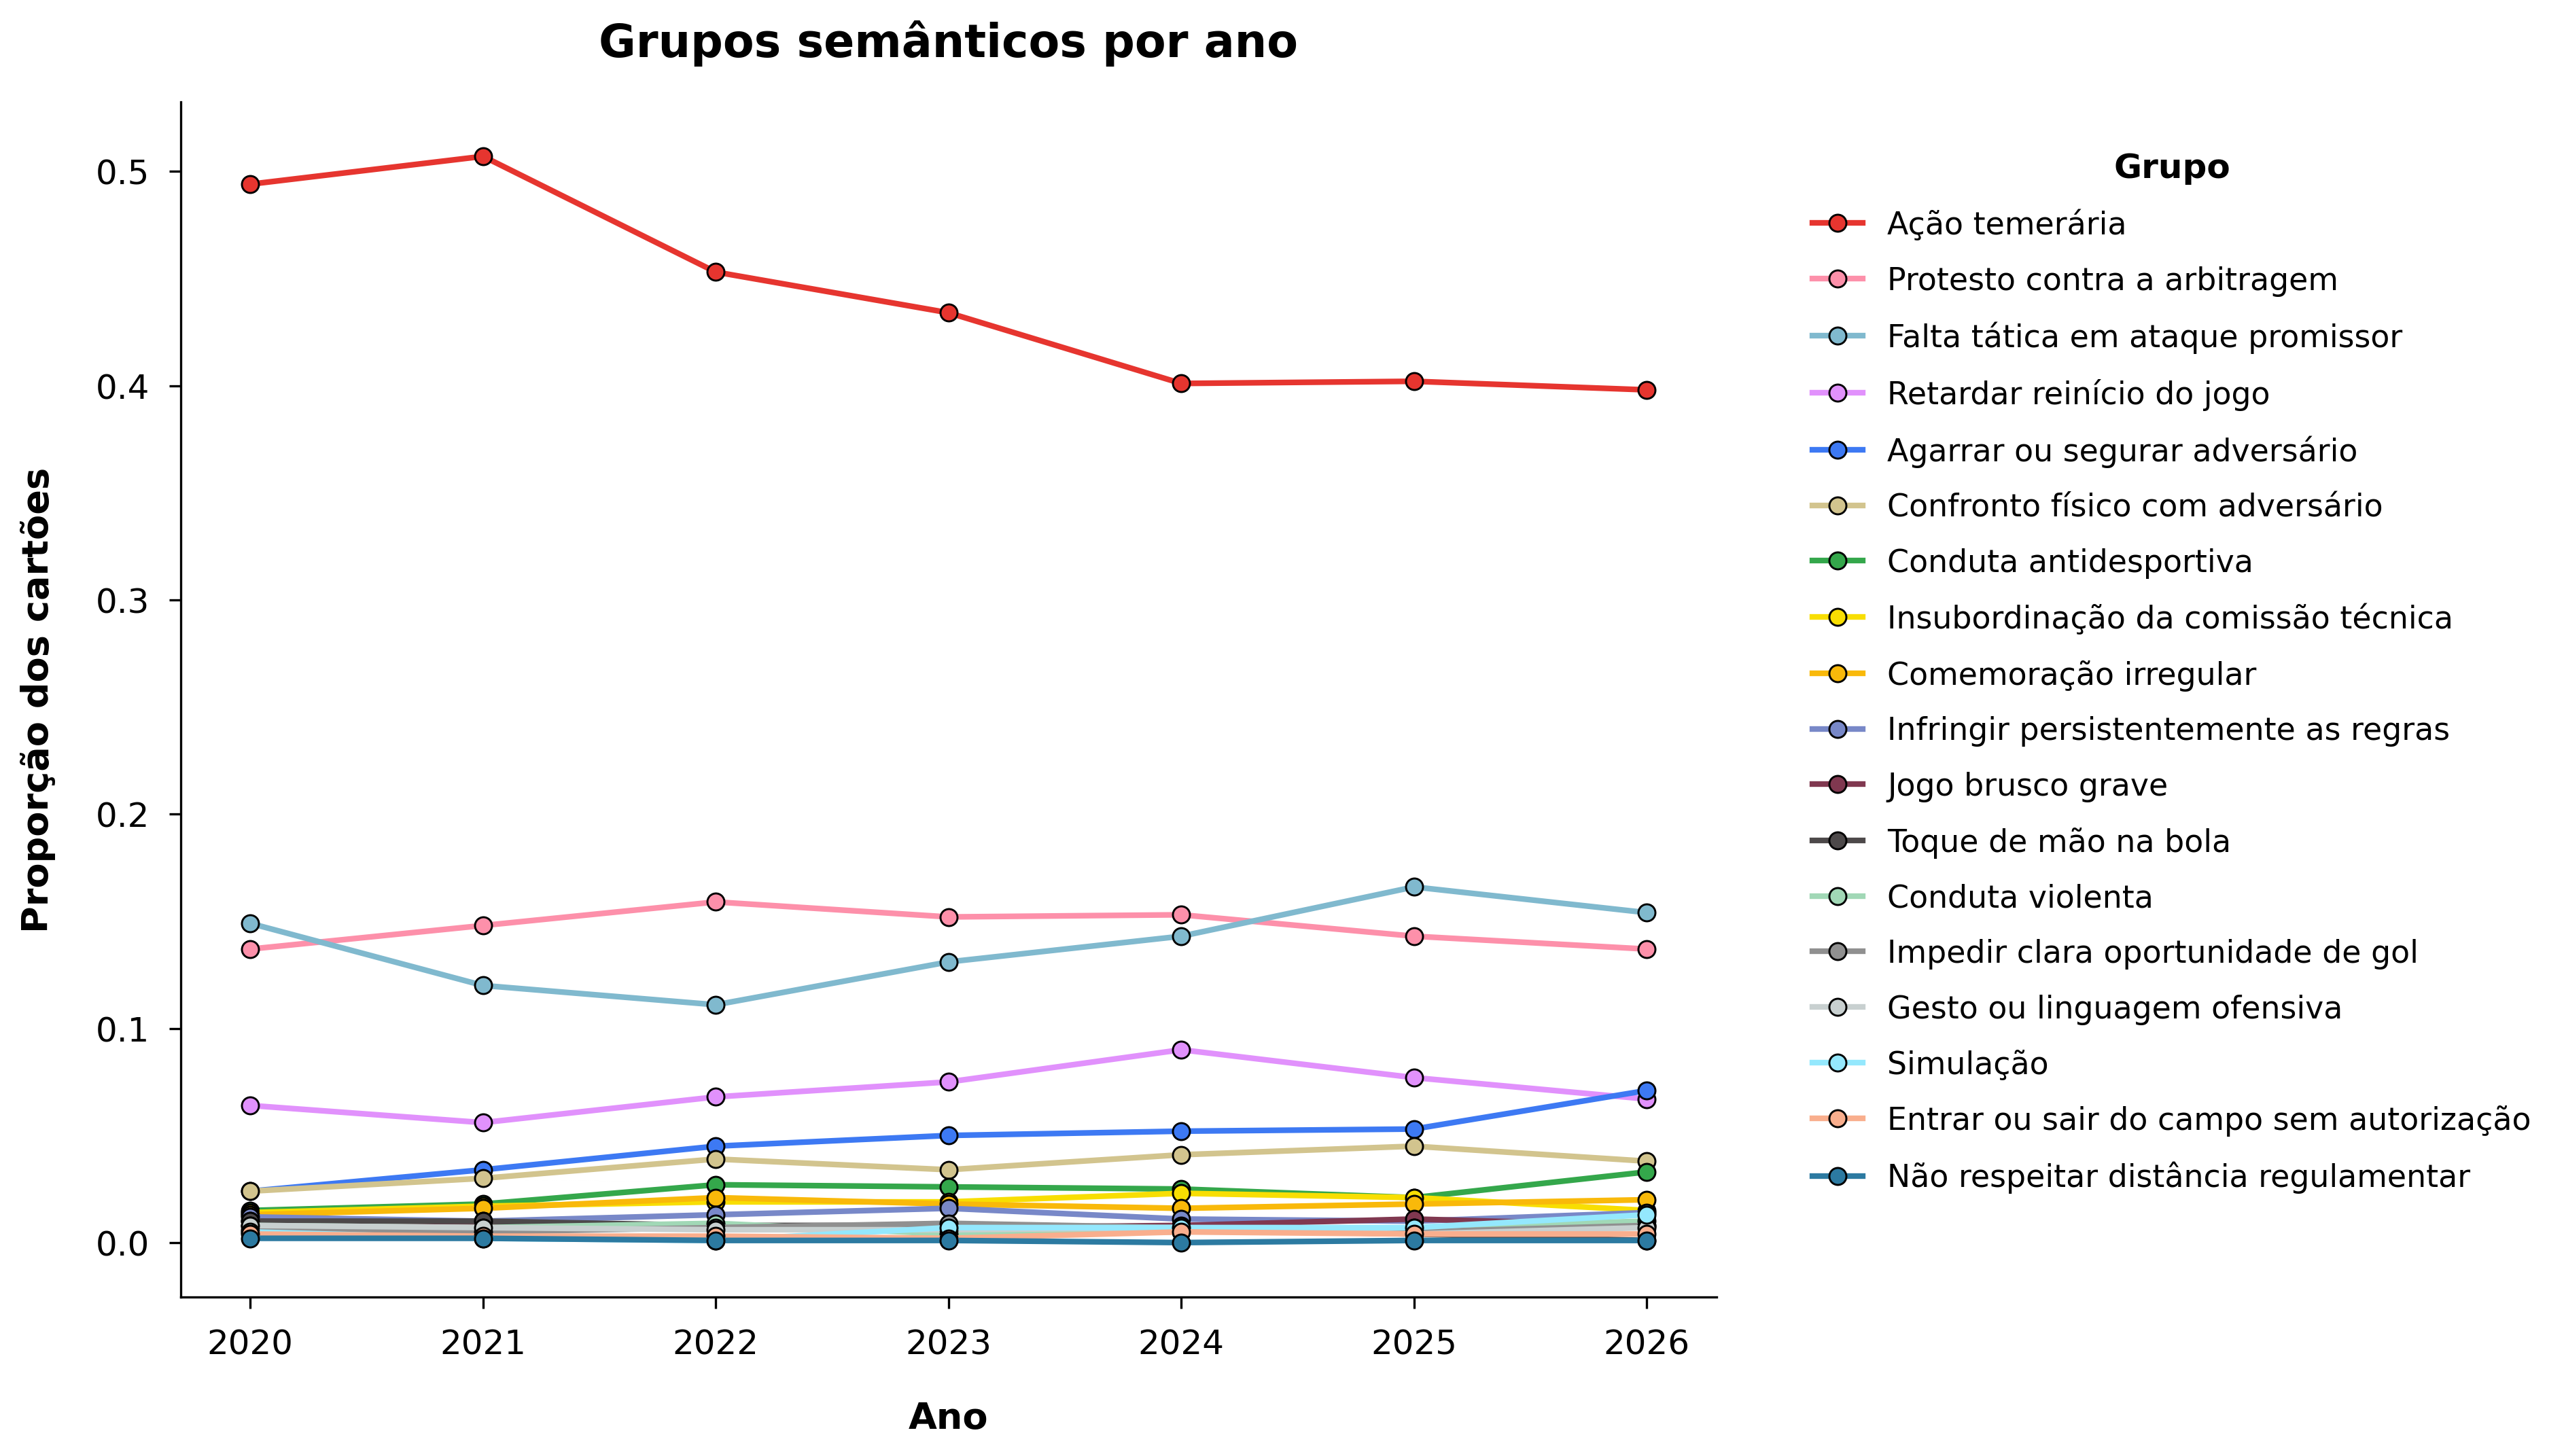
\includegraphics[width=\textwidth]{card_reason_groups_proportions_by_year.png}
  \fonte{Elaborado pelos autores.}
\end{figure}

\FloatBarrier

As Figuras~\ref{fig-byteam} e~\ref{fig-byreferee} mostram os perfis disciplinares por time e árbitro. Times com maior proporção de faltas táticas podem indicar padrão defensivo de interrupção de transições. Diferenças entre árbitros podem refletir estilo de condução e perfil das competições apitadas. Esses recortes servem como diagnóstico qualitativo.

\begin{figure}[!htp]
  \centering
  \caption{Perfil disciplinar dos times com mais partidas na base.}
  \label{fig-byteam}
  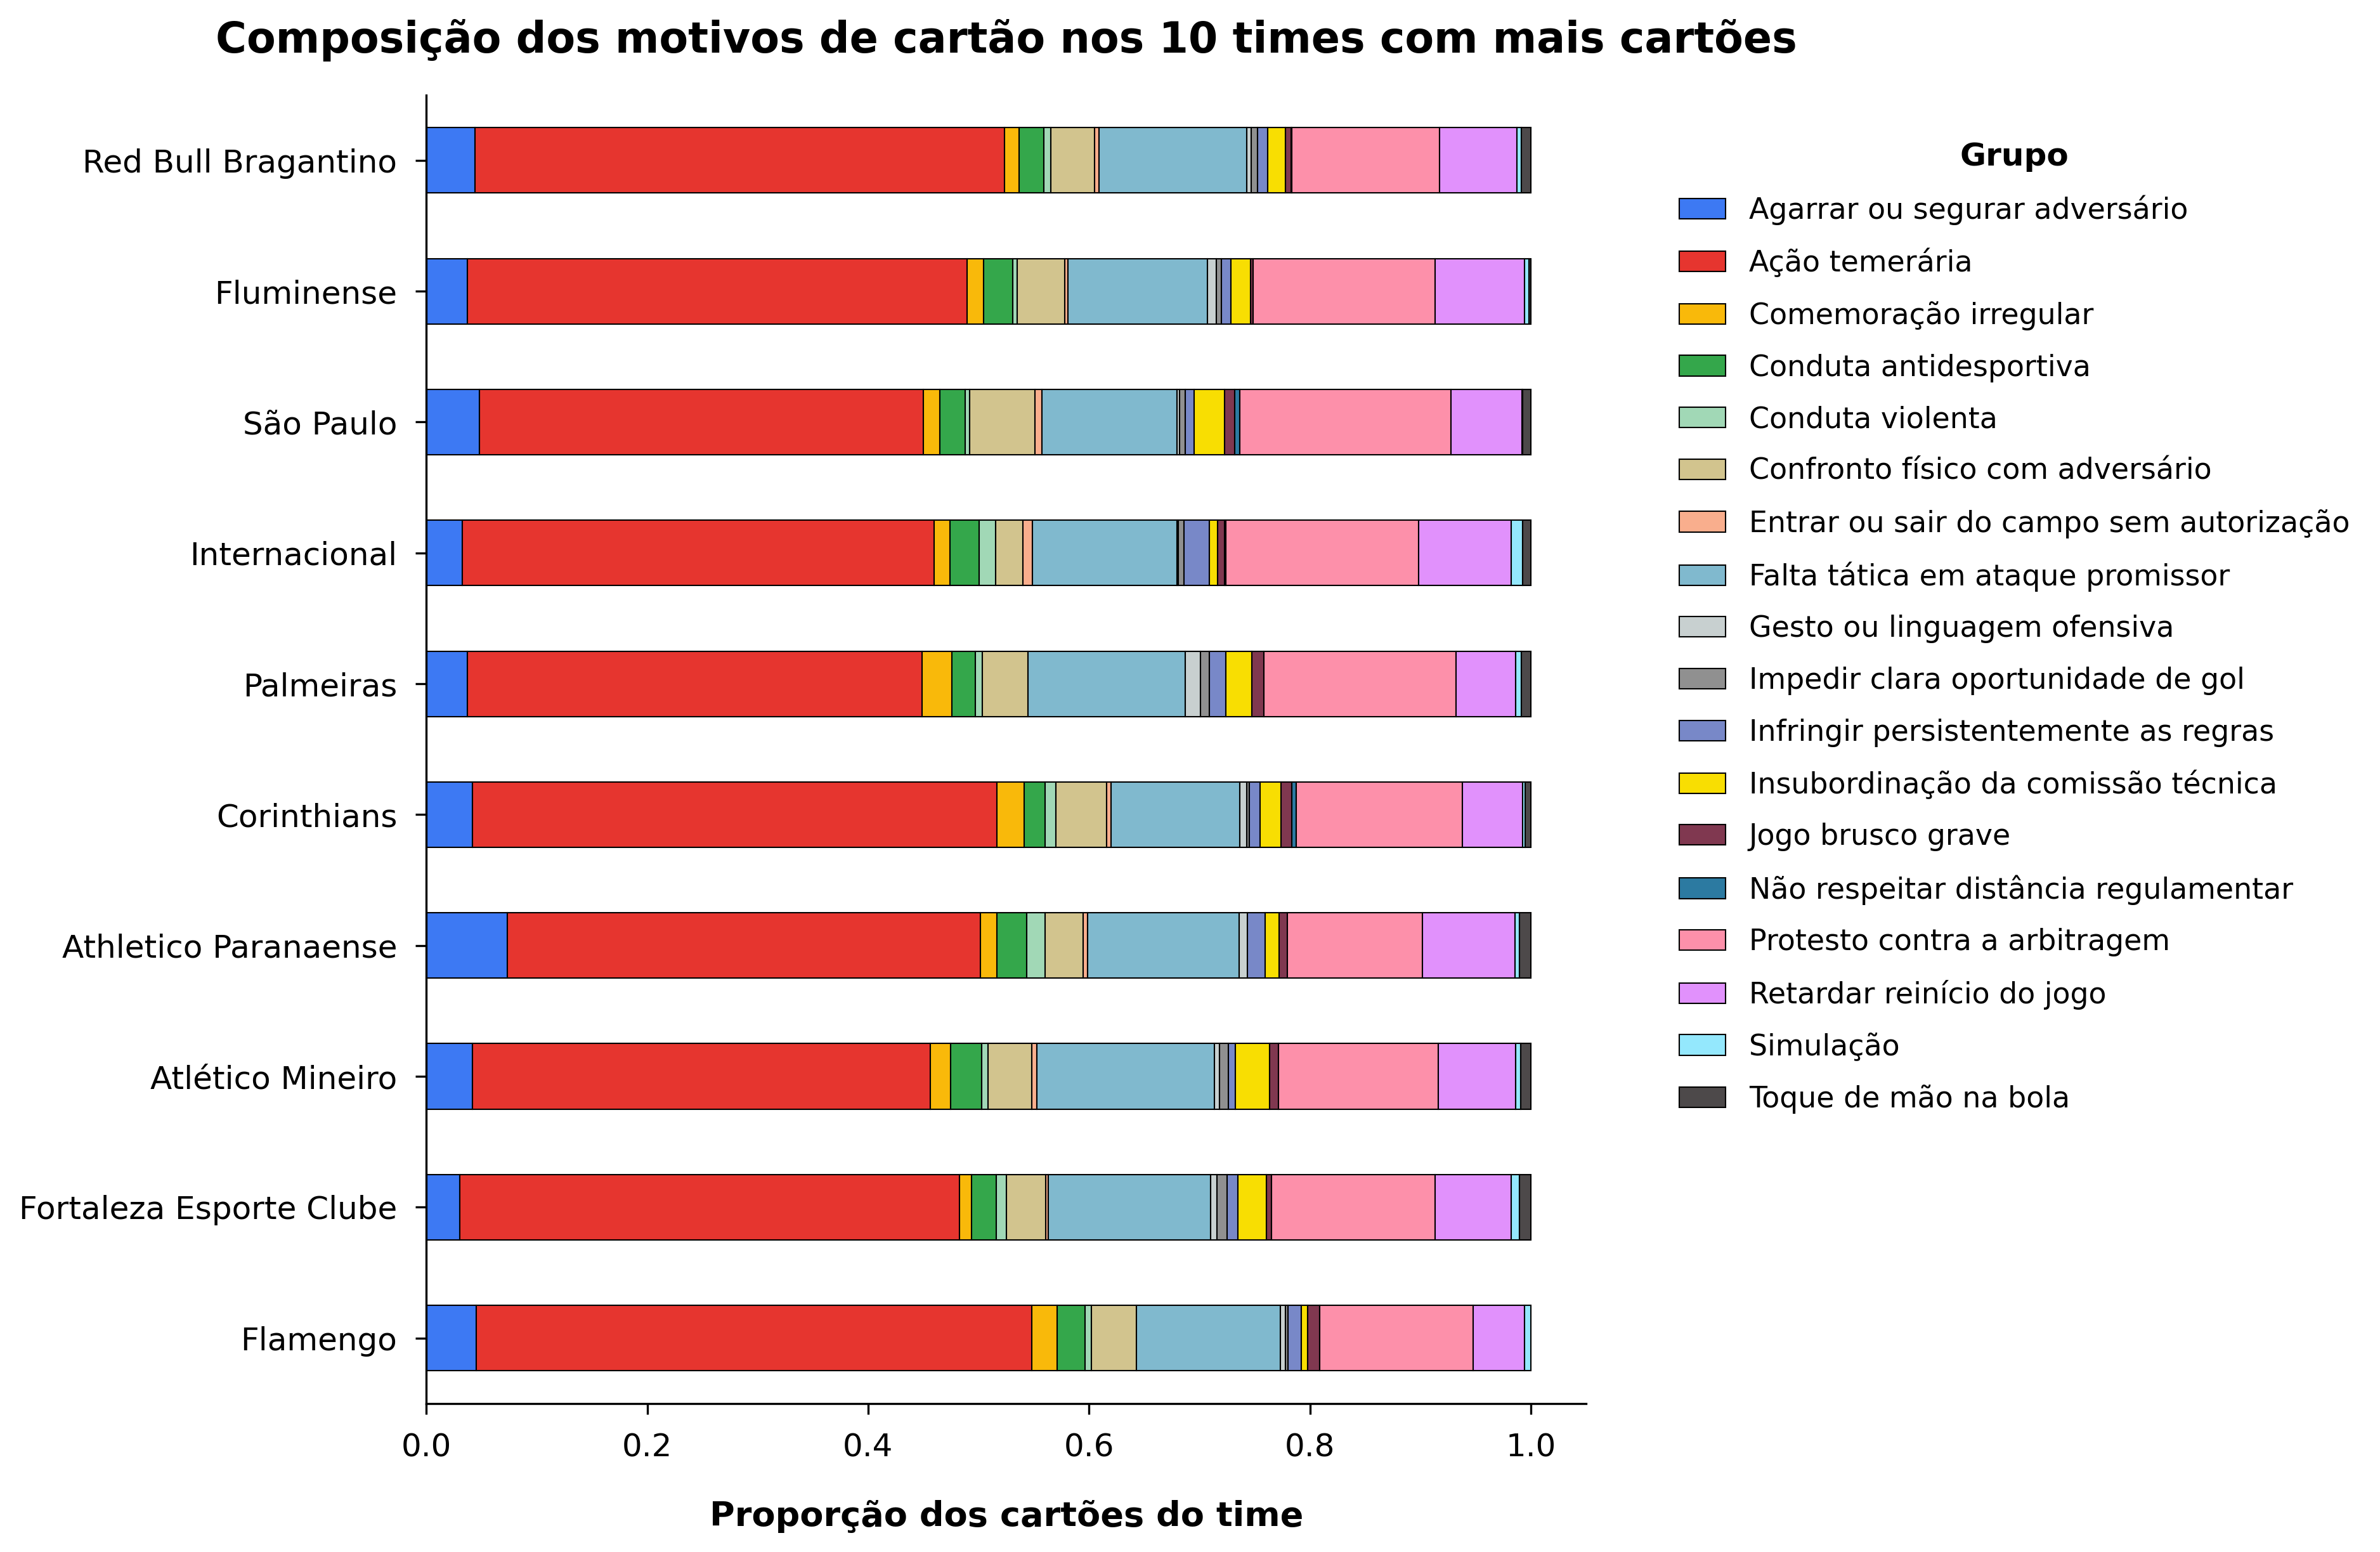
\includegraphics[width=0.8\textwidth]{card_reason_groups_by_team.png}
  \fonte{Elaborado pelos autores.}
\end{figure}

\begin{figure}[!htp]
  \centering
  \caption{Perfil disciplinar dos árbitros com mais partidas na base.}
  \label{fig-byreferee}
  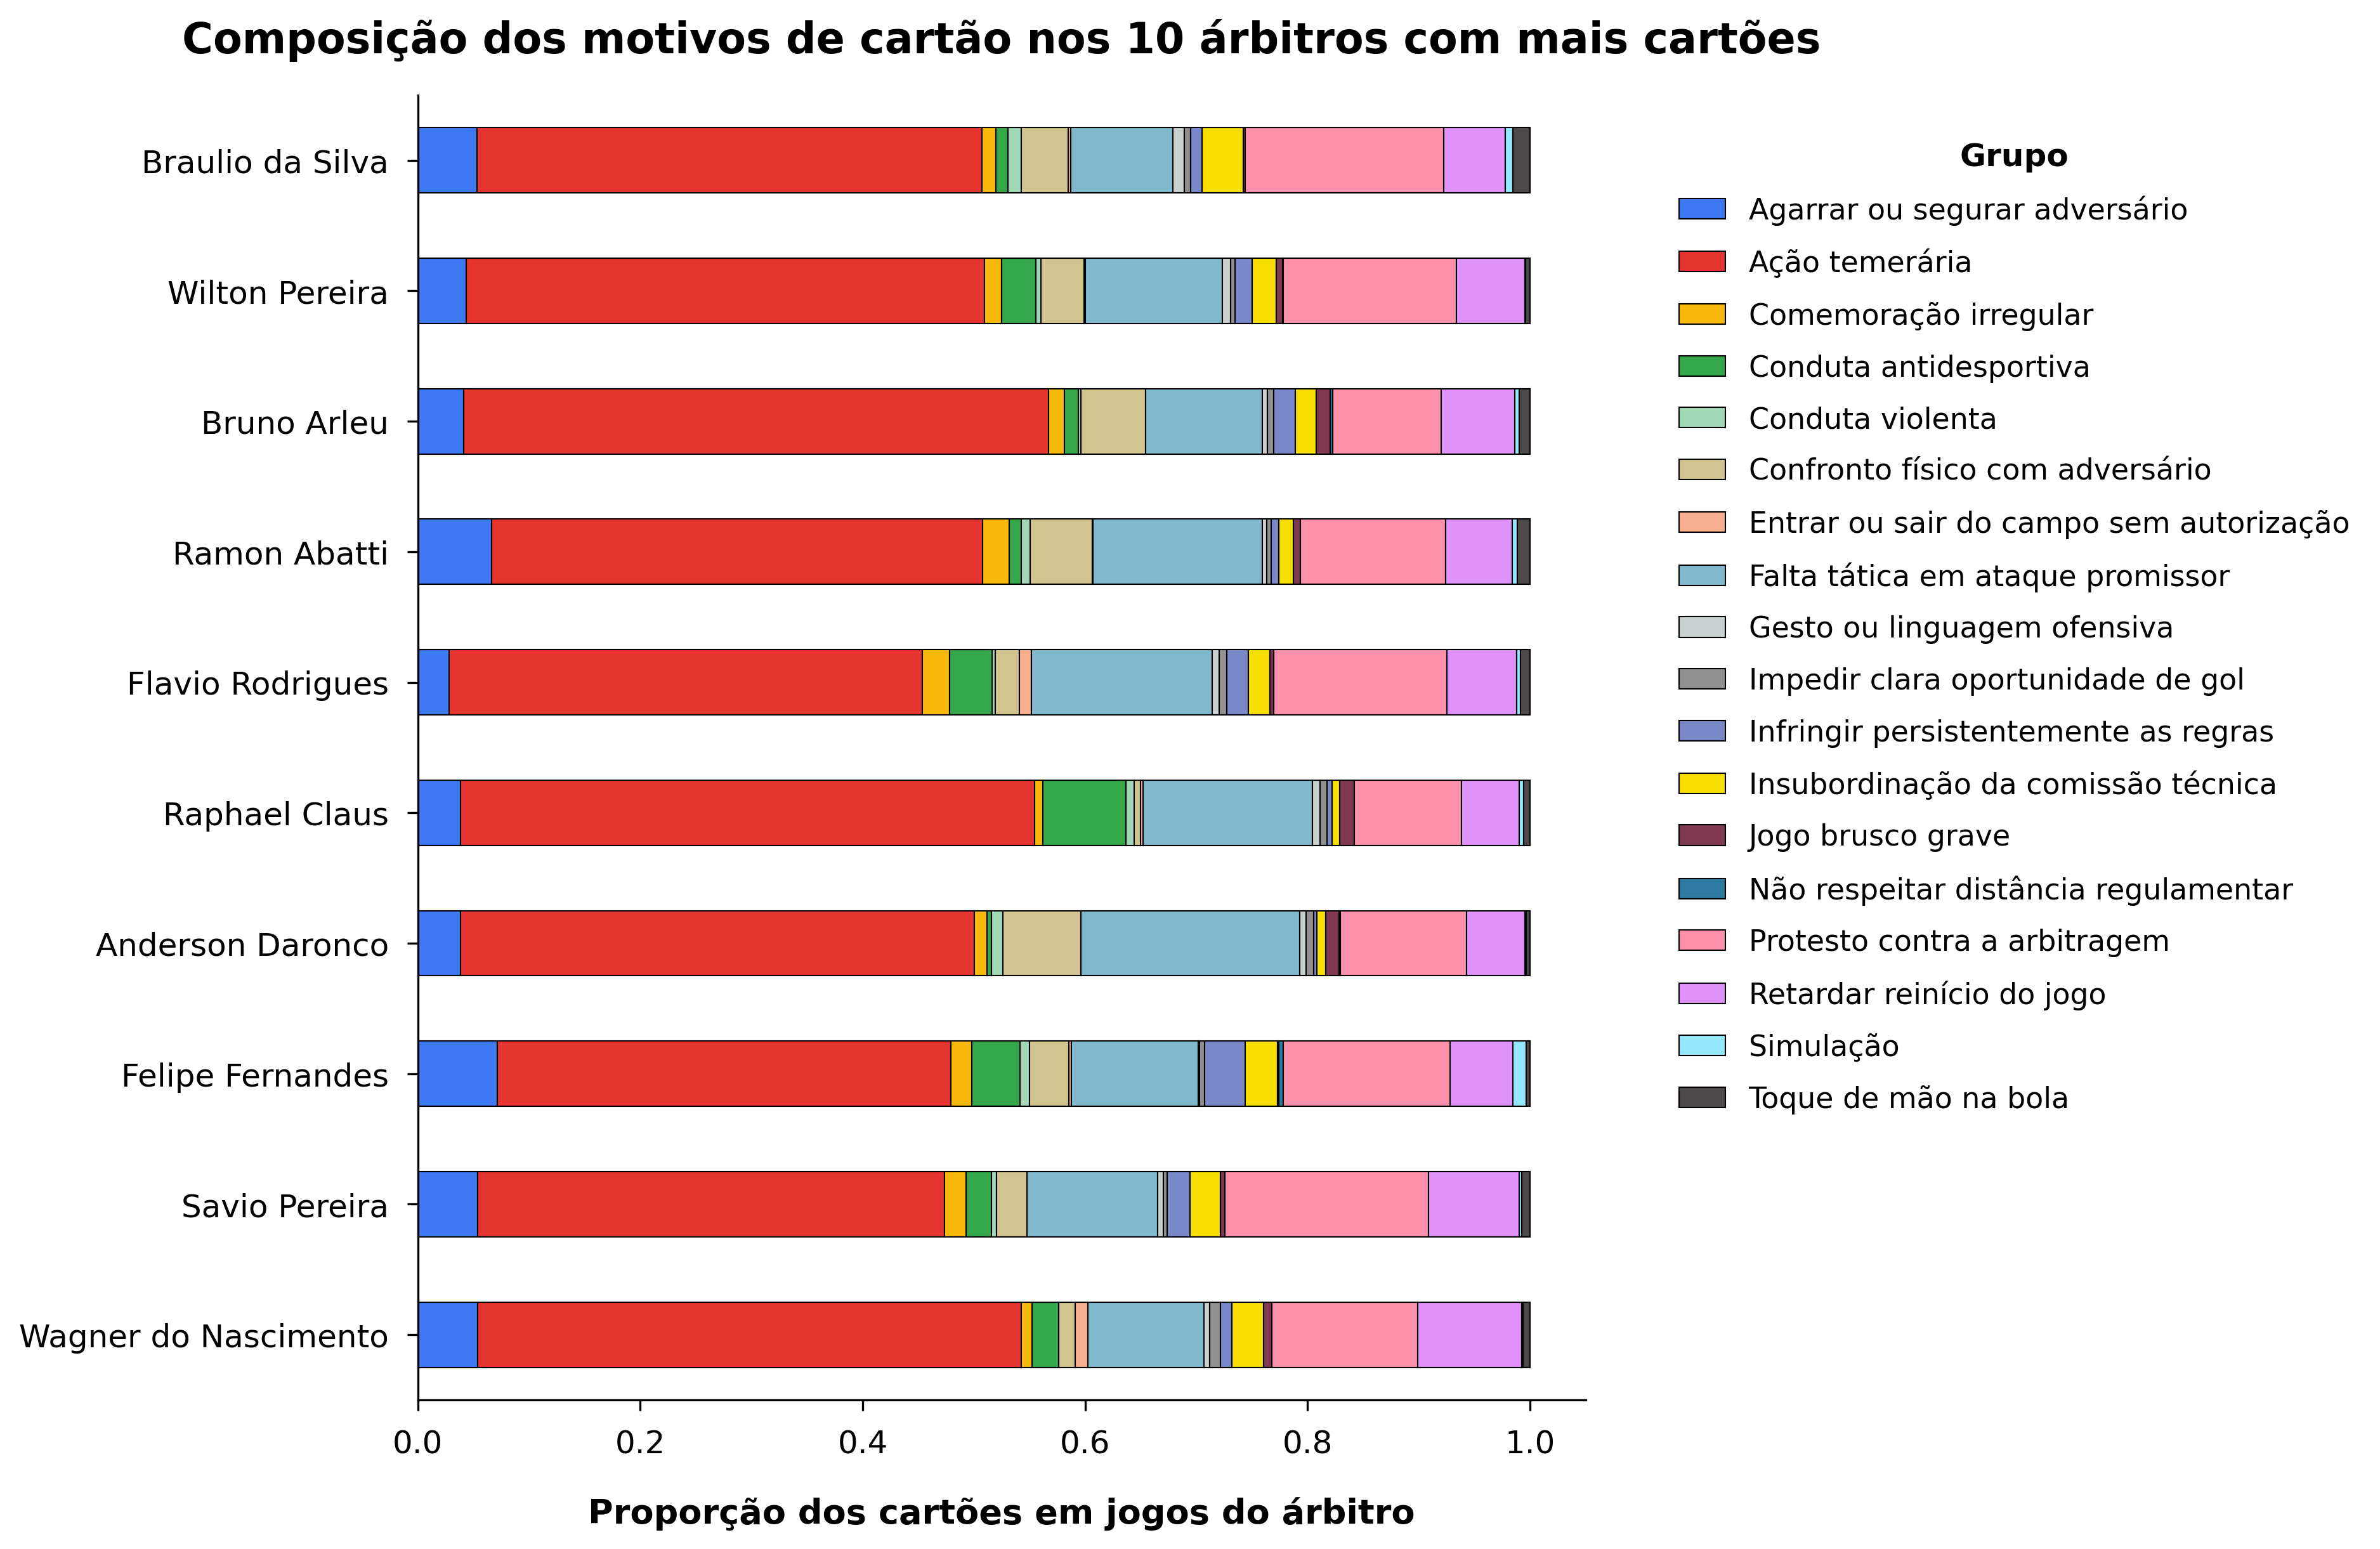
\includegraphics[width=0.8\textwidth]{card_reason_groups_by_referee.png}
  \fonte{Elaborado pelos autores.}
\end{figure}

\FloatBarrier

\section{Comparação entre Métodos}

\subsection{Score Médio de Coesão}

A Figura~\ref{fig-score-comparison} compara o score médio de coesão entre BERTopic e LLM zero-shot para cada grupo.

\begin{figure}[!htp]
  \centering
  \caption{Score médio por grupo: BERTopic versus LLM zero-shot.}
  \label{fig-score-comparison}
  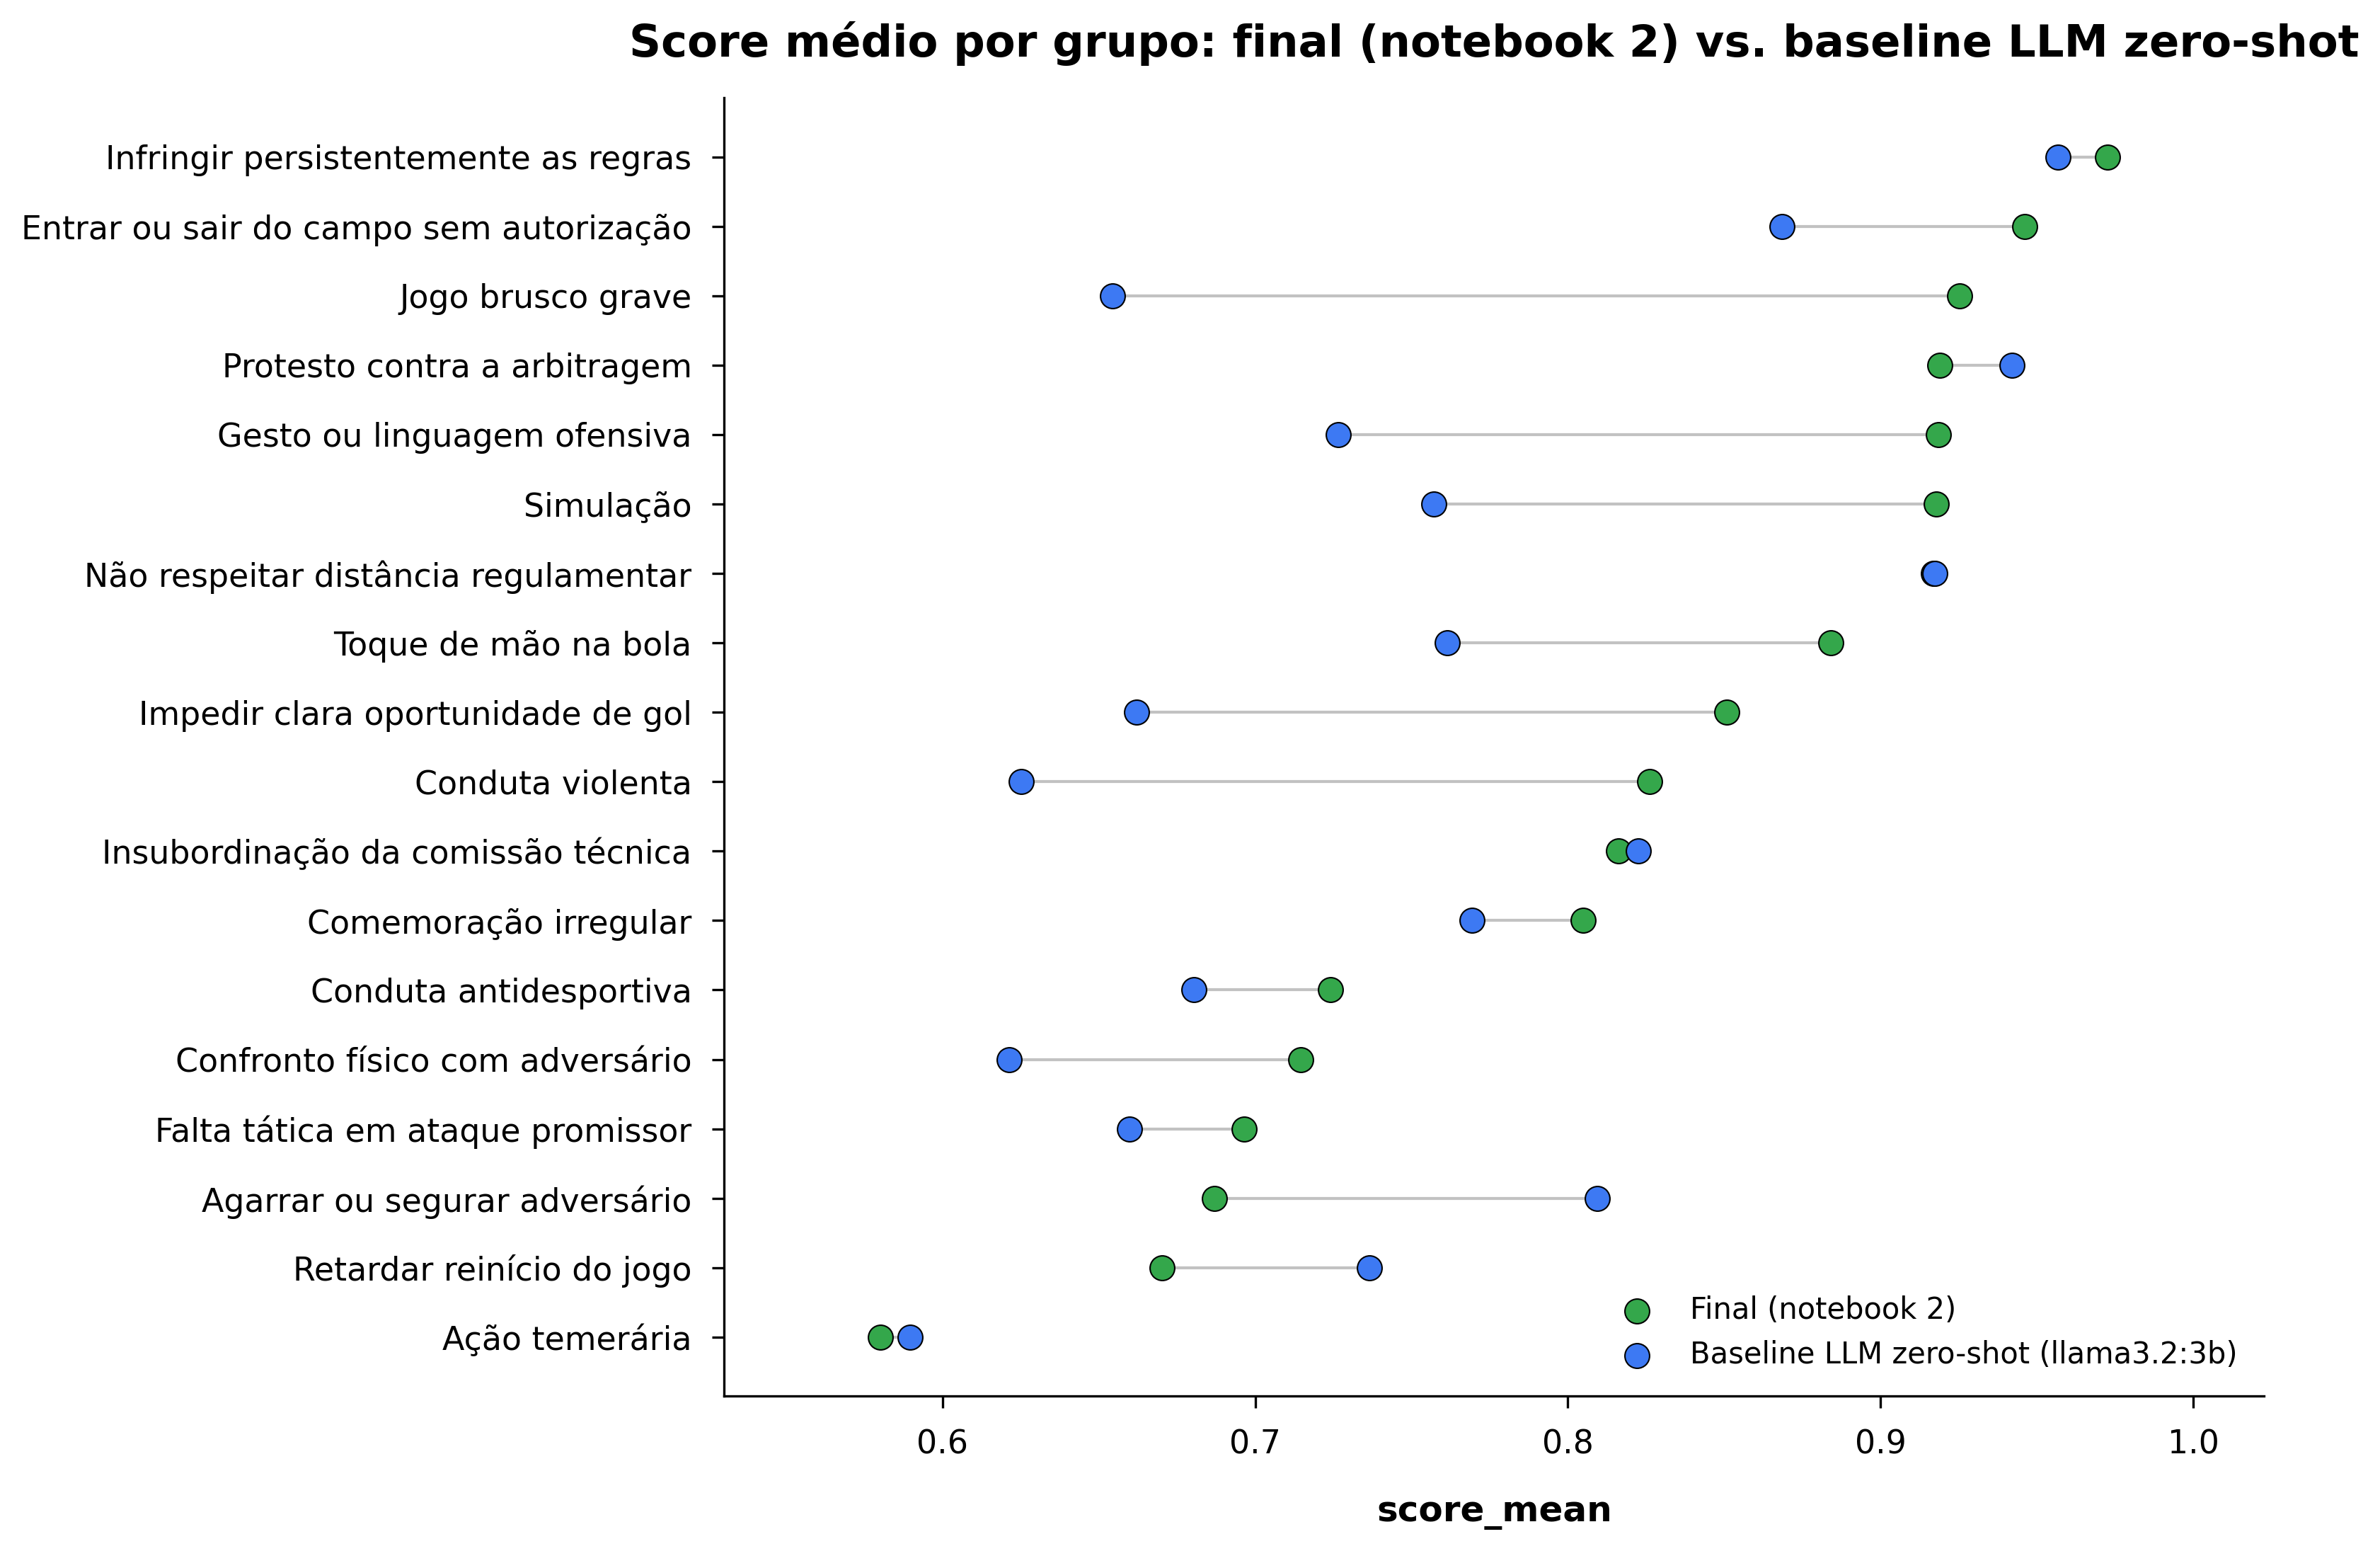
\includegraphics[width=0.8\textwidth]{baseline_llm_score_mean_by_group.png}
  \fonte{Elaborado pelos autores.}
\end{figure}

\FloatBarrier

O BERTopic supera a LLM zero-shot na maioria dos grupos. Grupos com vocabulário específico, como Retardar reinício do jogo e Infringir persistentemente as regras, têm scores próximos nos dois sistemas, indicando que os nomes das categorias já são suficientes para guiar a classificação nesses casos. Grupos com fronteiras menos nítidas, como Confronto físico com adversário e Conduta violenta, registram queda expressiva no score da LLM, confirmando que o fine-tuning é mais relevante onde a distinção entre categorias exige especialização no domínio.

\subsection{Recuperabilidade por Classificadores}

A Tabela~\ref{tab-retrieval} apresenta os resultados em validação cruzada com 5 folds. Os embeddings fine-tunados são os únicos atributos dos classificadores em ambos os experimentos.

\begin{table}[!htp]
  \centering
  \caption{Recuperabilidade dos rótulos BERTopic e LLM em 5-fold CV.}
  \label{tab-retrieval}
  \small
  \begin{tabular}{lrrrr}
    \toprule
    Classificador & \multicolumn{2}{c}{BERTopic} & \multicolumn{2}{c}{LLM zero-shot} \\
    \cmidrule(lr){2-3}\cmidrule(lr){4-5}
    & F1 Macro & Accuracy & F1 Macro & Accuracy \\
    \midrule
    KNN & 0,834 & 0,897 & 0,627 & 0,733 \\
    Regressão Logística & 0,859 & 0,919 & 0,584 & 0,751 \\
    SVM Linear & \textbf{0,882} & \textbf{0,933} & \textbf{0,652} & \textbf{0,771} \\
    \bottomrule
  \end{tabular}
  \fonte{Elaborado pelos autores.}
  \nota{Hiperparâmetros selecionados por F1 Macro no CV. Melhor modelo de cada sistema em negrito.}
\end{table}

\FloatBarrier

O SVM Linear atinge F1 Macro de 0,882 para BERTopic contra 0,652 para LLM, diferença de 0,230 pontos. A Figura~\ref{fig-retrieval-global} ilustra a comparação.

\begin{figure}[!htp]
  \centering
  \caption{F1 Macro e Accuracy dos três classificadores nos dois sistemas.}
  \label{fig-retrieval-global}
  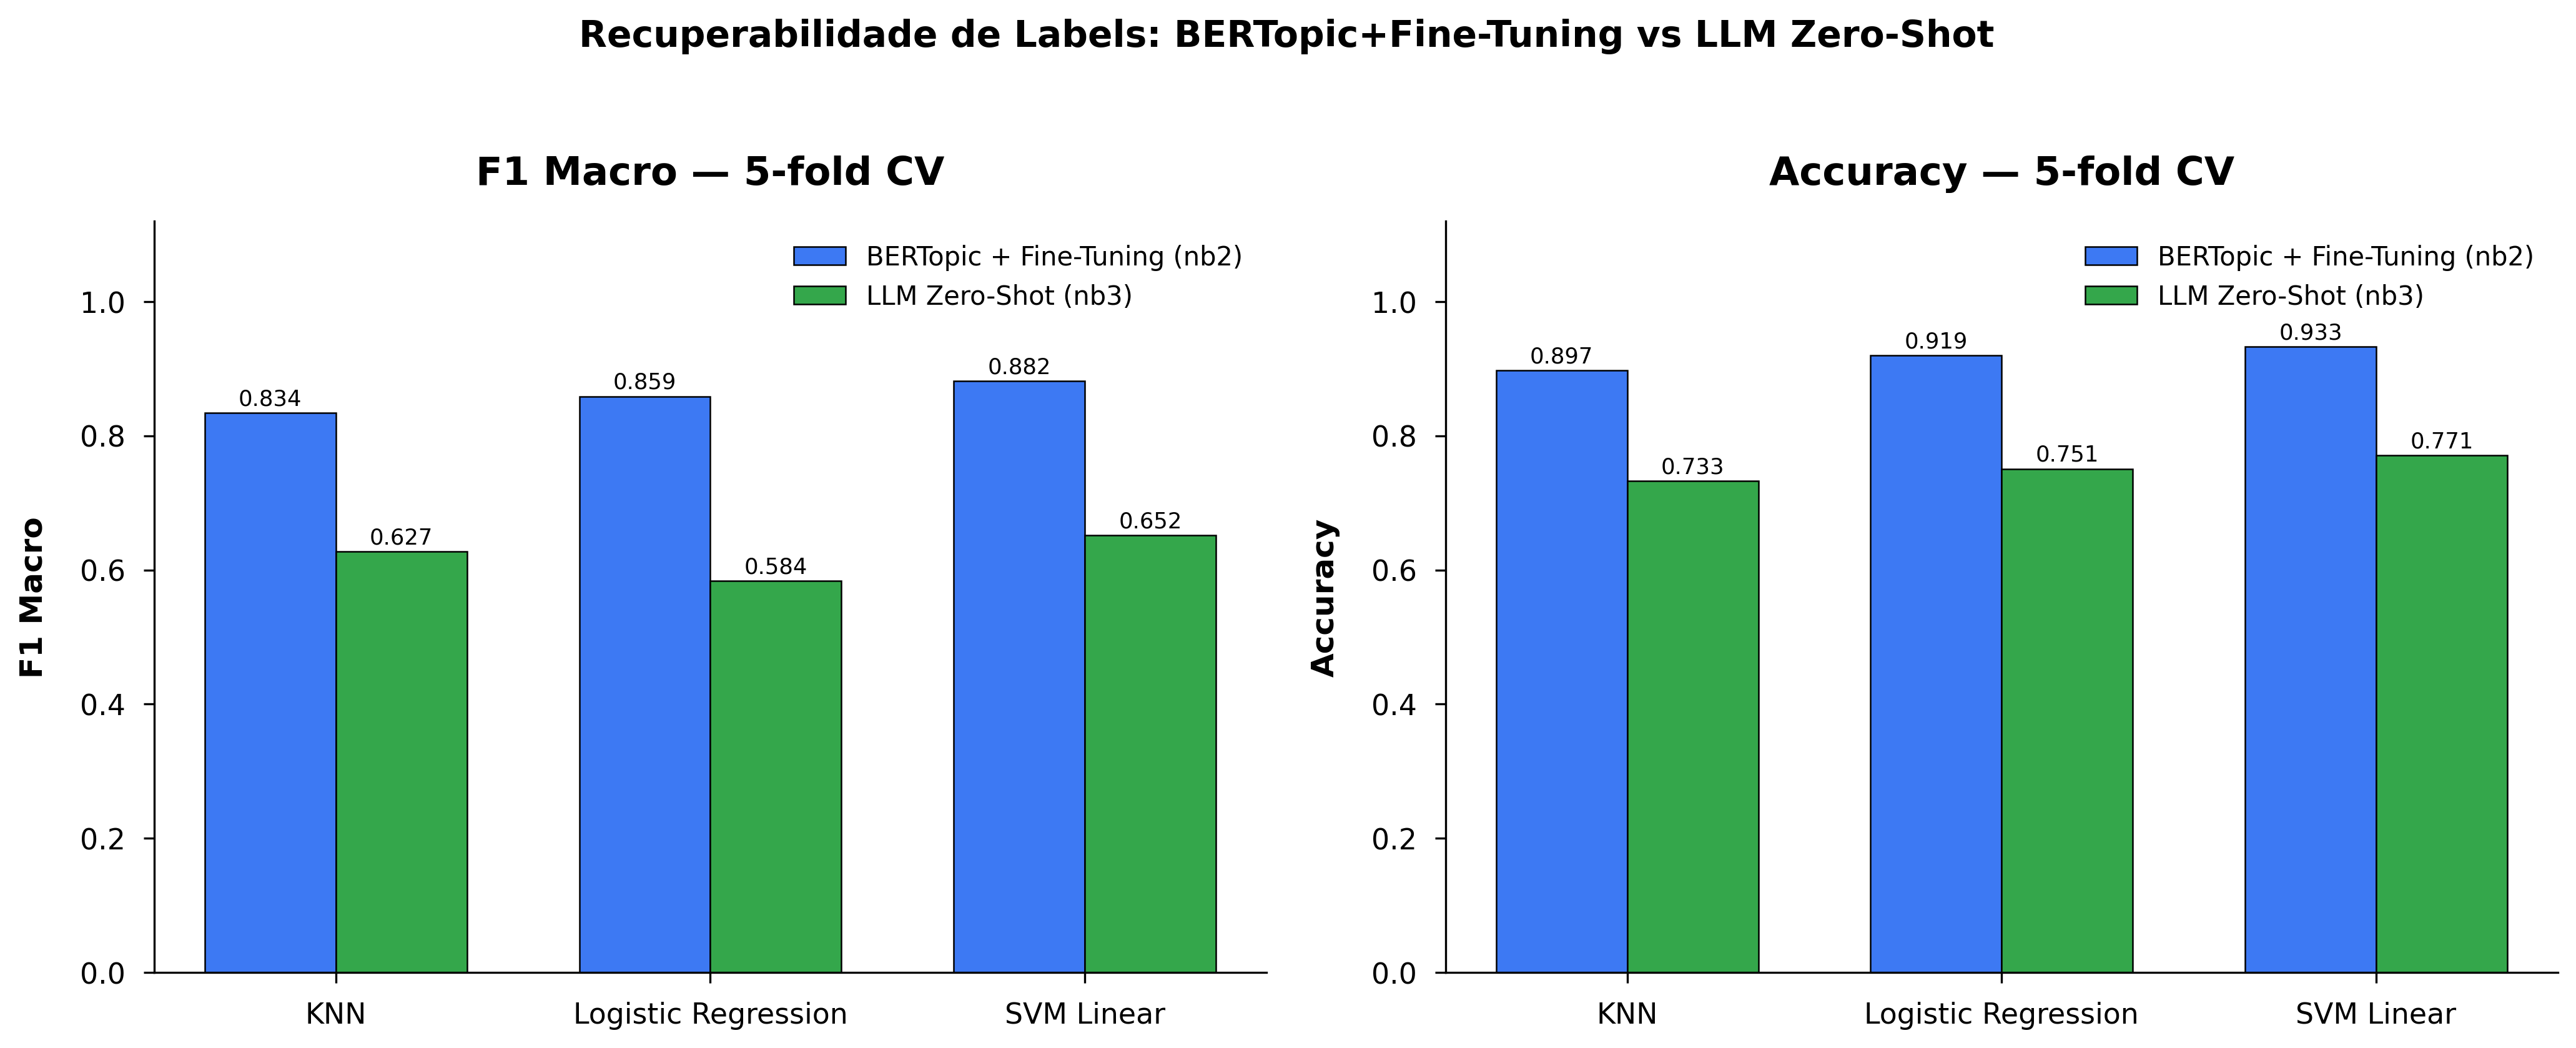
\includegraphics[width=\textwidth]{retrieval_nb2_vs_nb3_comparison.png}
  \fonte{Elaborado pelos autores.}
\end{figure}

\FloatBarrier

A Figura~\ref{fig-retrieval-grupo} mostra o F1 por grupo para o SVM Linear. No BERTopic, 15 dos 18 grupos atingem F1 acima de 0,80. As exceções são Conduta violenta (0,482), Conduta antidesportiva (0,763) e Jogo brusco grave (0,780), que compartilham vocabulário próximo. No sistema LLM, a distribuição é muito mais heterogênea: Gesto ou linguagem ofensiva chega a F1 de apenas 0,167.

\begin{figure}[!htp]
  \centering
  \caption{F1 por grupo para o SVM Linear: BERTopic versus LLM zero-shot.}
  \label{fig-retrieval-grupo}
  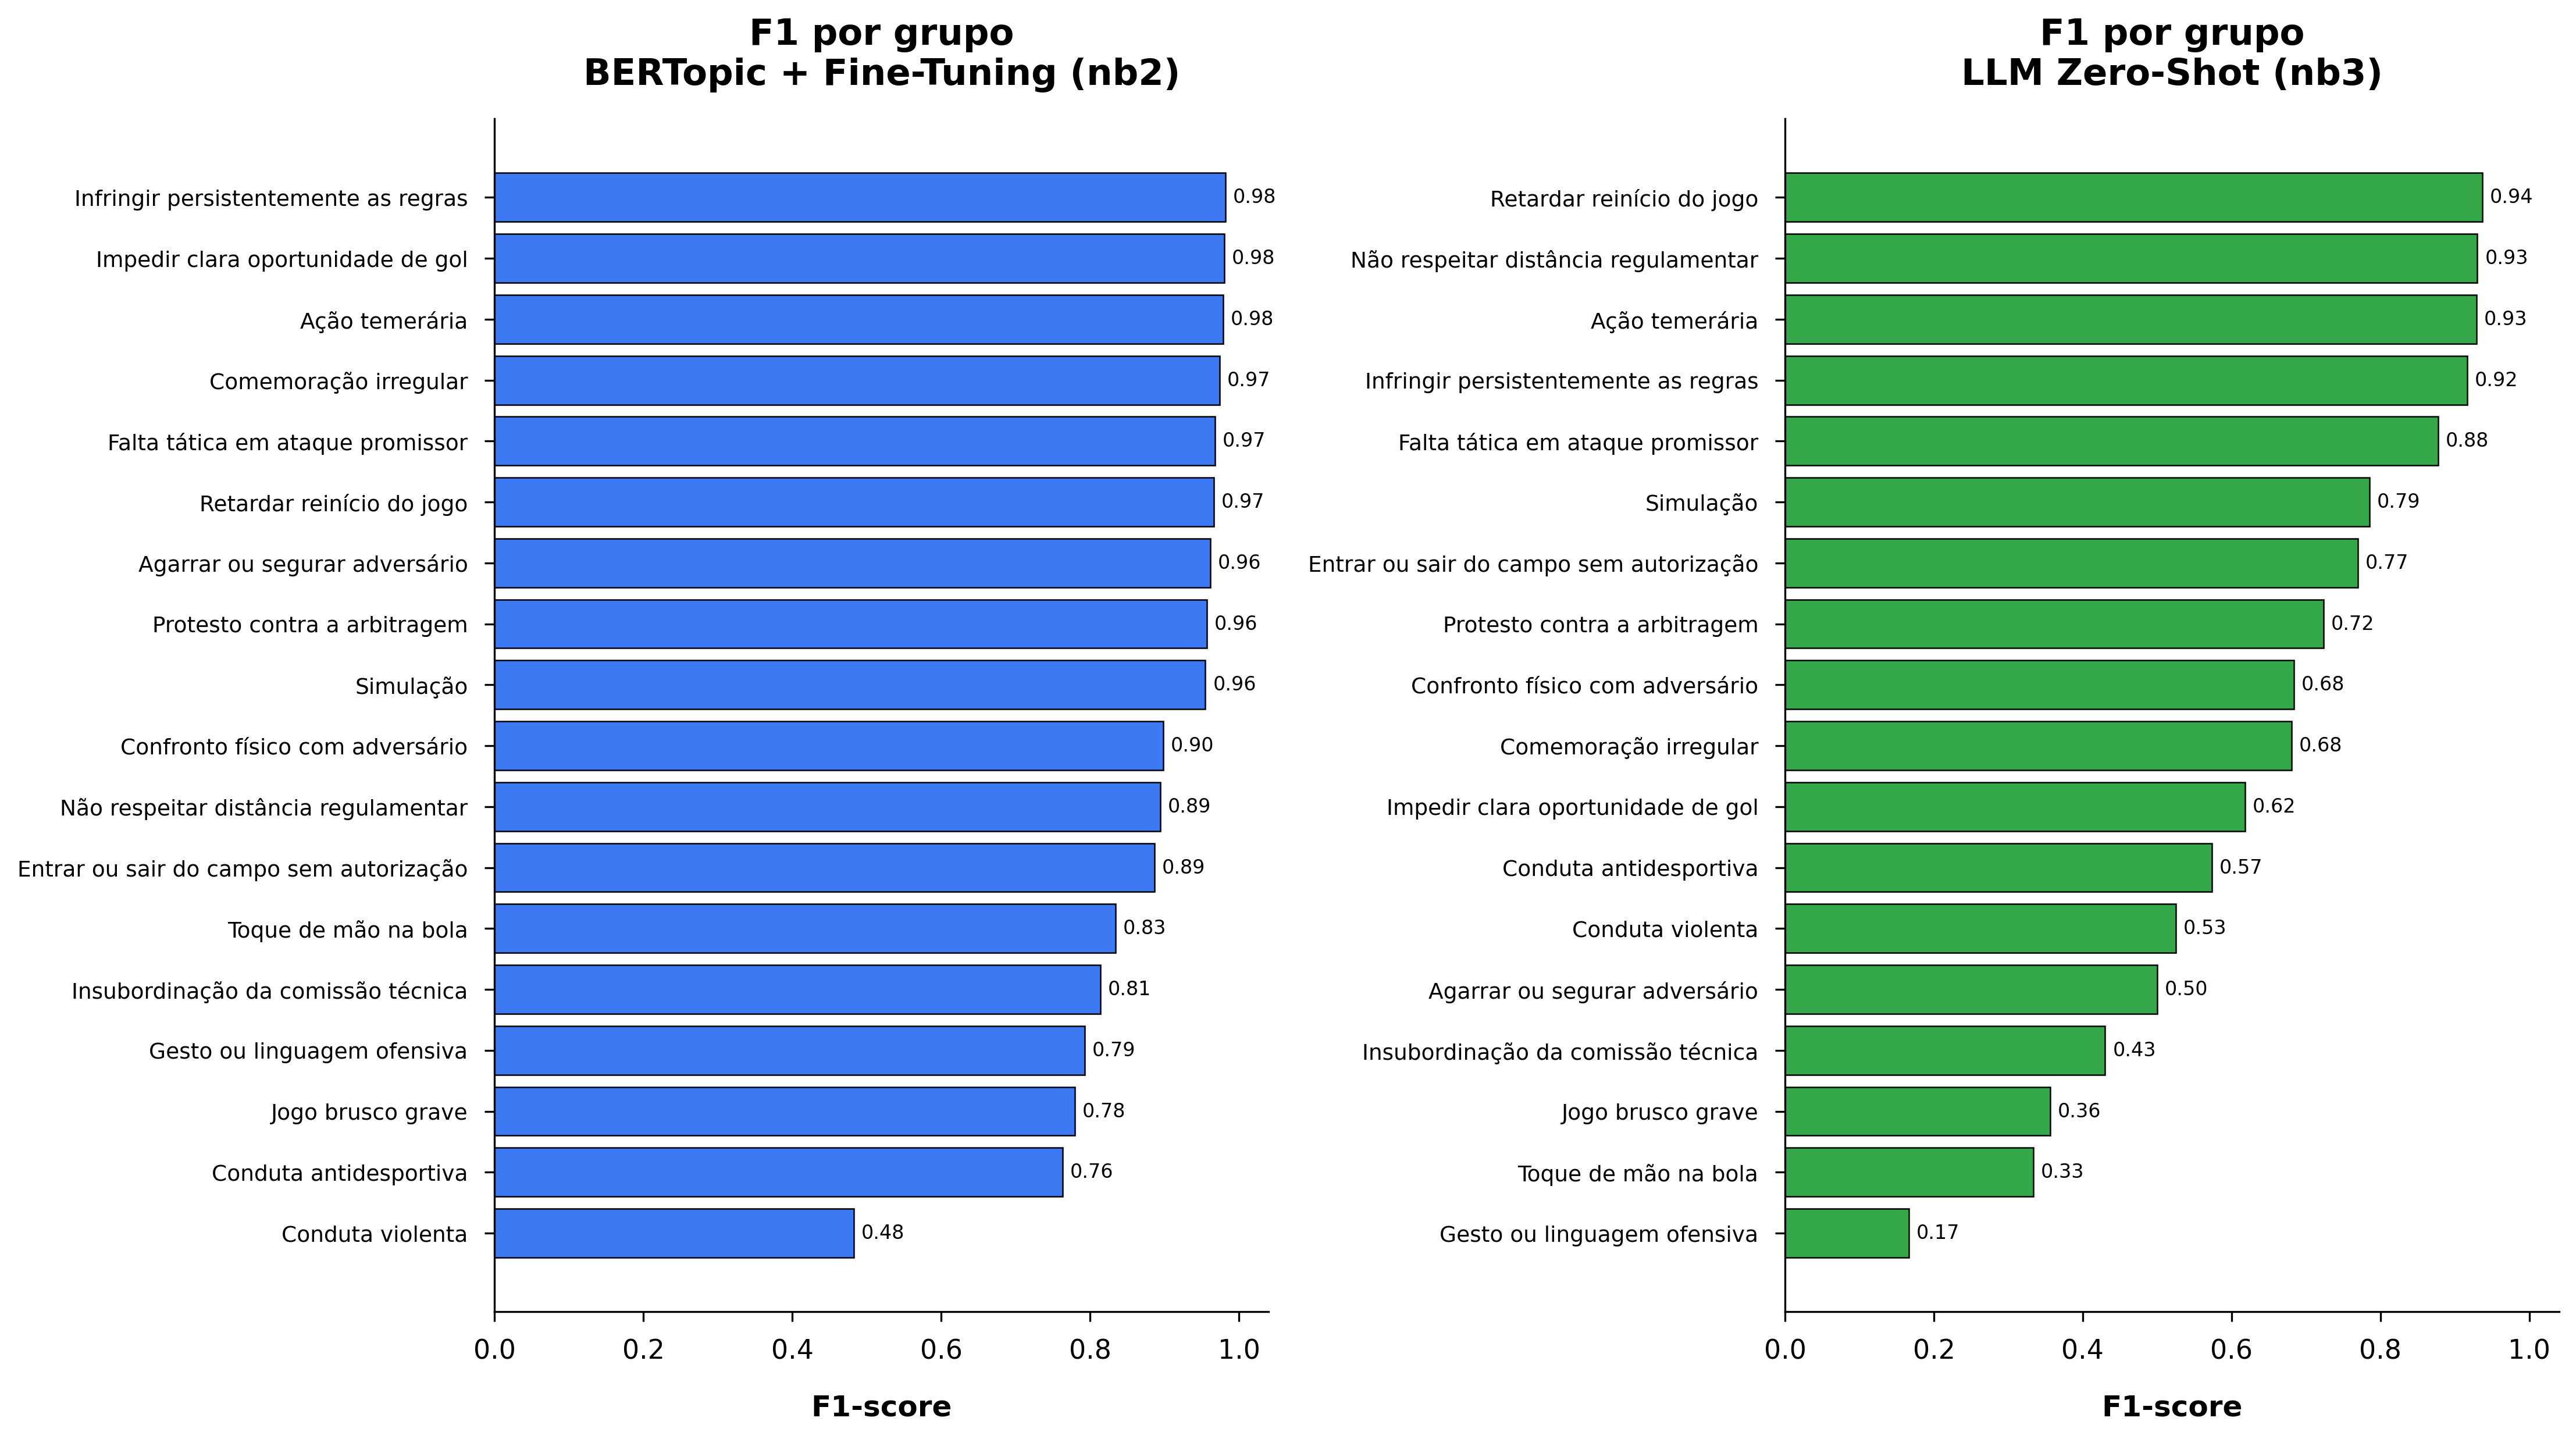
\includegraphics[width=\textwidth]{retrieval_f1_per_group_nb2_vs_nb3.png}
  \fonte{Elaborado pelos autores.}
\end{figure}

\FloatBarrier

\subsection{Concordância entre Sistemas}

A concordância direta entre BERTopic e LLM zero-shot é de 61,2\%. A Figura~\ref{fig-agreement} detalha a taxa por grupo.

\begin{figure}[!htp]
  \centering
  \caption{Taxa de concordância direta entre BERTopic e LLM zero-shot por grupo.}
  \label{fig-agreement}
  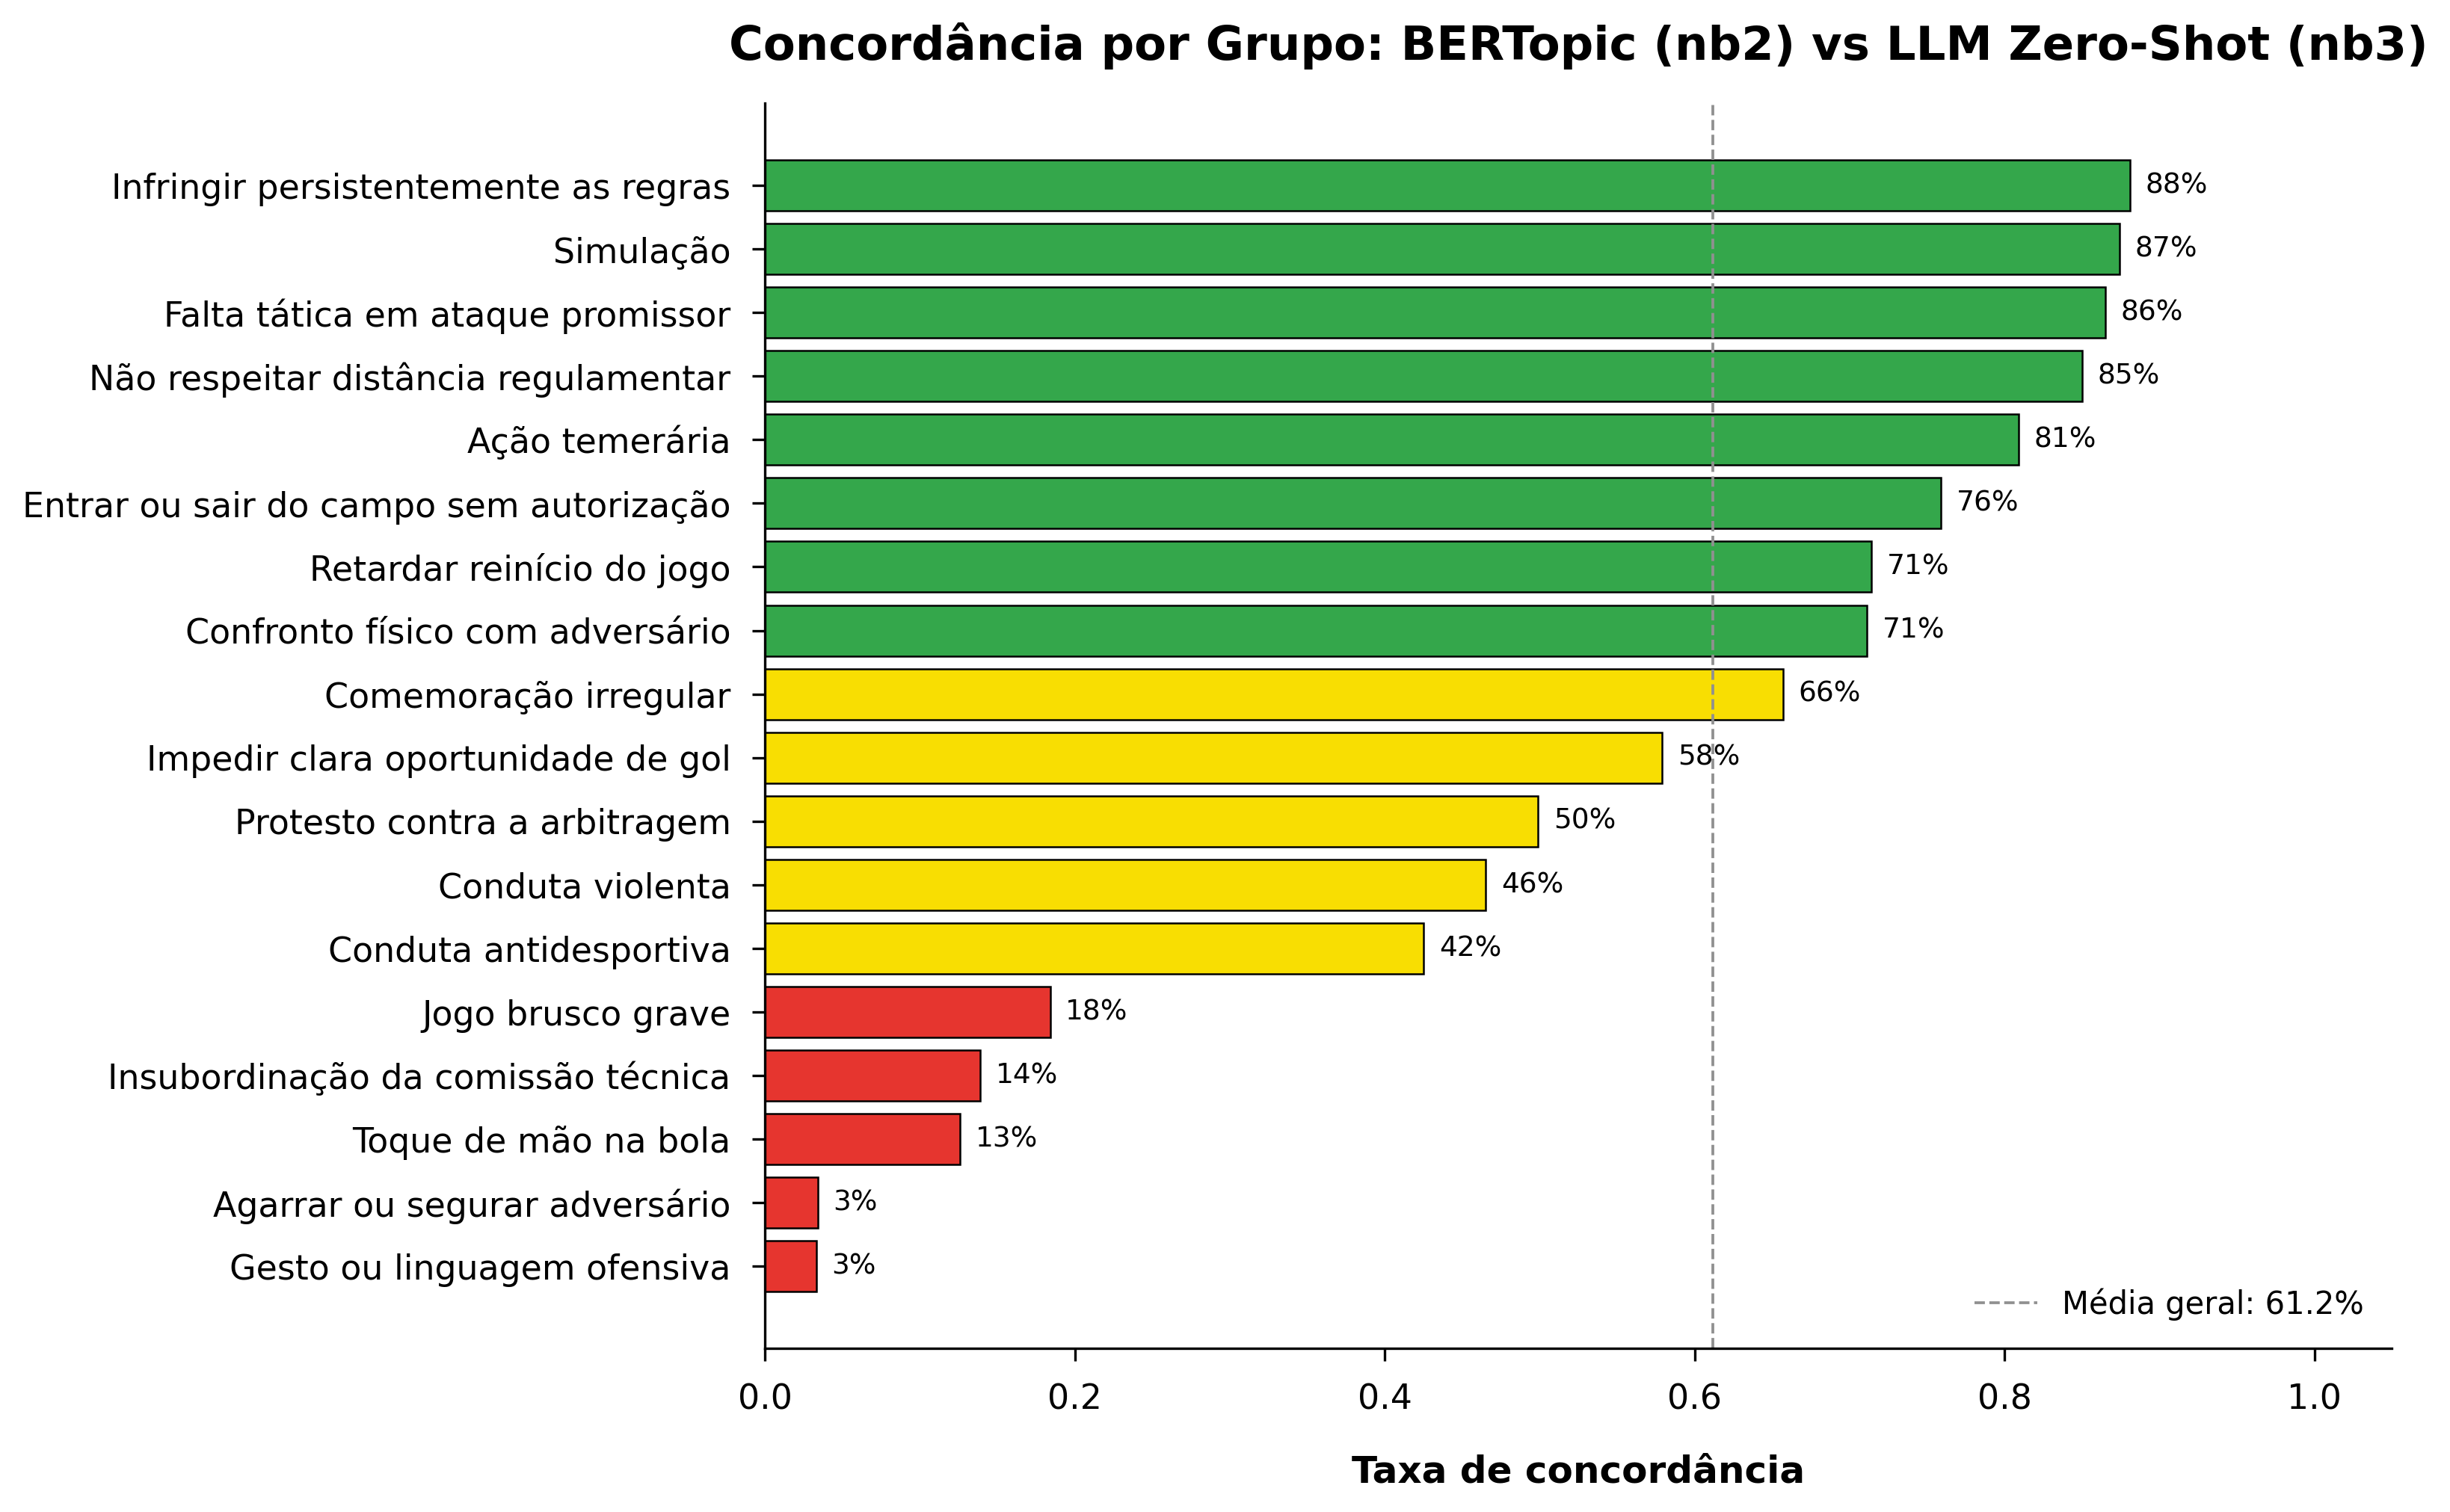
\includegraphics[width=0.92\textwidth]{retrieval_agreement_by_group.png}
  \fonte{Elaborado pelos autores.}
\end{figure}

\FloatBarrier

Grupos como Infringir persistentemente as regras (88,1\%), Simulação (87,4\%) e Falta tática em ataque promissor (86,5\%) têm alta concordância por possuírem vocabulário não ambíguo. Os grupos com concordância abaixo de 15\%, Agarrar ou segurar adversário (3,4\%) e Gesto ou linguagem ofensiva (3,3\%), são aqueles em que a LLM usa categorias mais amplas como substitutos. O maior par de divergência é Ação temerária (BERTopic) contra Confronto físico com adversário (LLM), com 297 textos: a LLM classifica pelo contato físico descrito, sem distinguir a temeridade intencional, separação que o BERTopic faz com base na geometria dos embeddings.

% =============================================================================
\chapter{Conclusão}
% =============================================================================

Este trabalho desenvolveu um pipeline de NLP para classificação semântica de justificativas de cartões em súmulas da CBF. O método combina embeddings multilinguais com BERTopic em duas passagens e fine-tuning contrastivo auto-supervisionado, produzindo uma taxonomia de 18 grupos disciplinares alinhados com as Leis do Jogo da IFAB.

O fine-tuning produziu ganho mensurável: DBCV aumentou 21,7\% e a taxa de outliers caiu 6,2 pontos percentuais. A comparação com a baseline LLM zero-shot confirmou a vantagem do pipeline especializado: o SVM Linear atinge F1 Macro de 0,882 sobre os rótulos BERTopic contra 0,652 sobre os rótulos da LLM, diferença de 0,230. A concordância direta de 61,2\% mostra que a LLM captura as categorias com vocabulário mais nítido, mas não reproduz as distinções taxonômicas finas do pipeline.

Entre os padrões disciplinares encontrados, Ação temerária concentra 44,4\% dos cartões.

\section{Limitações}

A qualidade da extração depende do formato dos PDFs, e variações de layout ao longo dos anos podem causar erros de parsing em um subconjunto de documentos. A taxonomia manual introduz decisões subjetivas nos casos limítrofes entre grupos com vocabulário próximo, como Conduta violenta, Jogo brusco grave e Ação temerária. A baseline LLM foi avaliada apenas com o modelo \textit{llama3.2:3b}, de pequeno porte, e modelos maiores poderiam ter desempenho diferente.

\section{Extensões Futuras}

Extensões naturais incluem aplicar o pipeline a competições estaduais, investigar a evolução de grupos específicos em resposta a mudanças nas Leis do Jogo e explorar a relação entre perfil disciplinar de árbitros e resultados de partidas. Modelos de linguagem maiores poderiam ser avaliados como baseline zero-shot. Aprendizado ativo poderia reduzir o esforço de rotulagem manual em iterações futuras, priorizando revisão humana nos textos mais próximos das fronteiras entre grupos.

\postextual

\bibliography{USPSC-bib/USPSC-modelo-references}

\end{document}
